% RECUERDA QUE ESTA ES LA PLANTILLA NUEVA

% Config
\documentclass{article}
\usepackage[utf8]{inputenc}

% Paquetes
\usepackage{multicol}
\usepackage[a4paper, left=1in, right=1in, top=1in, bottom=1in, includehead, headheight=3mm]{geometry}
\usepackage{amsfonts, amsthm, amssymb, amsmath}
\usepackage{xcolor}
\usepackage{mathtools}
\usepackage[pdfusetitle]{hyperref}
\usepackage{ninecolors}
\usepackage{graphicx}
\usepackage{enumitem}


\hypersetup{colorlinks=true, linkcolor=black, urlcolor=black}

\title{Título}
\author{}
\date{}

% Comandos
\newcommand{\newlines}{\newline\newline}

\begin{document}

\section*{Series $\mathbf{n}^{\circ} 1$: Wave Packet}

\begin{enumerate}
    \item Consider a one-dimensional wave function defined at $t=0$ as the superposition of 3 plane waves:

    $$
    \psi(x, 0) = A\left(e^{i k_{0} x} + \frac{1}{2} e^{i\left(k_{0}-\frac{\Delta k}{2}\right) x} + \frac{1}{2} e^{i\left(k_{0}+\frac{\Delta k}{2}\right) x}\right)
    $$

    \begin{enumerate}
        \item What should be the dimension of $A$?

        \textcolor{red}{Solution: $A \equiv [L]^{-\frac{d}{2}}$}

        \item For which values of $x$ is the probability density $|\psi(x, 0)|^{2}$ maximal? null?

        \textcolor{red}{Solution: $|\psi(x, 0)|^{2} = A A^{*}\left(\cos \left(\frac{\Delta k}{2} x\right) + 1\right)^{2}$ is maximal if $x = n \frac{4 \pi}{\Delta k}$ and minimal (null) if $x = \frac{2 \pi}{\Delta k} + n \frac{4 \pi}{\Delta k}$}

        \item Let $\Delta x$ be the distance between two consecutive zeros of $|\psi(x, 0)|^{2}$, what relation links $\Delta x$ and $\Delta k$?

        \textcolor{red}{Solution: $\Delta x \Delta k = 4 \pi$}
    \end{enumerate}

    \item We are now interested in the superposition of an infinity of plane waves. The distribution of wave vectors $k$ at $t=0$ is defined by

    $$
    \begin{aligned}
    & \tilde{\psi}(k, 0) = \frac{1}{\sqrt{\Delta k}} \text{ if } k_{0} - \frac{\Delta k}{2} \leq k \leq k_{0} + \frac{\Delta k}{2} \\
    & \tilde{\psi}(k, 0) = 0 \text{ elsewhere }
    \end{aligned}
    $$

    \begin{enumerate}
        \item Calculate the corresponding wave function $\psi(x, 0)$.

        \textcolor{red}{Solution: $\psi(x, 0) = \sqrt{\frac{\Delta k}{2 \pi}} e^{i k_{0} x} \operatorname{sinc}\left(\frac{\Delta k}{2} x\right)$}

        \item Estimate the characteristic widths $\Delta x$ and $\Delta k$ of $|\psi(x, 0)|^{2}$ and $|\tilde{\psi}(k, 0)|^{2}$ and the product $\Delta x \Delta k$.

        \textcolor{red}{Solution: $\Delta x \Delta k = 4 \pi$ (for $\Delta x =$ central lobe of the sinc function. $2 \pi$ otherwise)}
    \end{enumerate}

    \item Here are three forms of wave functions corresponding to different quantum mechanics problems. For each of them, determine the constant $A$ so that it is normalized. We will need a mathematical tool that we will use regularly. Show that (hint: calculate $I^{2}$ by switching to polar coordinates):

    $$
    I = \int_{-\infty}^{+\infty} e^{-\alpha x^{2}} dx = \sqrt{\frac{\pi}{\alpha}}
    $$

    \begin{enumerate}
        \item $\psi(x) = A e^{i k_{0} x} e^{-x^{2} / 4 a^{2}}$ (Gaussian wave packet)

        \item $\psi(x) = A x e^{-m \omega x^{2} / 2 \hbar}$ (first excited state of the harmonic oscillator)

        \item $\psi(\vec{r}) = A e^{-r / a_{0}}$ where $r = ||\vec{r}||$ (ground state of the hydrogen atom) (! problem in 3D)

    \end{enumerate}
        {\color{red}Solution:
        \begin{enumerate}
            \item $A = \left(2 \pi a^{2}\right)^{-\frac{1}{4}}$

            \item $A = \left(\frac{4 m^{3} \omega^{3}}{\pi \hbar^{3}}\right)^{\frac{1}{4}}$

            \item $A = \left(\pi a_{0}^{3}\right)^{-\frac{1}{2}}$
        \end{enumerate}}

    \item Consider the Gaussian wave packet defined in 3(a) (at $t=0$)

    \begin{enumerate}
        \item Calculate the Fourier transform $\tilde{\psi}(k, 0)$ of $\psi(x, 0)$.

        \textcolor{red}{Solution: $\tilde{\psi}(k, 0) = \left(\frac{2 a^{2}}{\pi}\right)^{\frac{1}{4}} e^{-a^{2}\left(k-k_{0}\right)^{2}}$}

        \item Represent $|\tilde{\psi}(k, 0)|^{2}$. What is its shape? Where is the center of the wave packet?

        \textcolor{red}{Solution: $|\tilde{\psi}(k, 0)|^{2} = \sqrt{\frac{2 a^{2}}{\pi}} e^{-2 a^{2}\left(k-k_{0}\right)^{2}}$ it is a normalized Gaussian centered at $k_{0}$. It loses a factor $e^{-1 / 2}$ for $\Delta k = k - k_{0} = \frac{1}{2 a}$.}

        \item Calculate the widths $\Delta x$ and $\Delta k$ of $|\psi(x, 0)|^{2}$ and $|\tilde{\psi}(k, 0)|^{2}$ and the product $\Delta x \Delta k$.

        \textcolor{red}{Solution: $|\psi(x, 0)|^{2} = \sqrt{\frac{1}{2 \pi a^{2}}} e^{-\frac{x^{2}}{2 a^{2}}}$ it is a normalized Gaussian centered at $x=0$. It loses a factor $e^{-1 / 2}$ for $\Delta x = a$.}

        $$
        \Rightarrow \quad \Delta x \Delta k = \frac{1}{2}
        $$
    \end{enumerate}

    \item We are now interested in the dynamics of the previous Gaussian wave packet. The dispersion relation is given by $\omega = \hbar k^{2} / 2 m$.

    \begin{enumerate}
        \item Calculate the form of $\psi(x, t)$ and show that at time $t$ the wave packet remains Gaussian.

        \textcolor{red}{Solution: We must write the wave function as a superposition of plane waves:

        $$
        \psi(x, t) = \frac{1}{\sqrt{2 \pi}} \int_{-\infty}^{+\infty} \tilde{\psi}(k, 0) e^{-i(\omega t - k x)} dk \quad \text{with} \quad \omega = \frac{\hbar k^{2}}{2 m}
        $$

        As before, the idea is to make the Gaussian integral appear by factoring the argument of the exponential:
        $a^{2}\left(k-k_{0}\right)^{2} + i \frac{\hbar k^{2}}{2 m} t - i k x = K^{2} - \beta$ where $K$ depends linearly on $k$ and $\beta$ does not depend on it.
        After a somewhat tedious calculation, we obtain for the wave function:

        $$
        \psi(x, t) = \left(\frac{a^{2}}{2 \pi}\right)^{\frac{1}{4}} \frac{1}{u} \exp \left(-\frac{a^{2}}{4\left|u^{2}\right|^{2}}\left[\left(x - \frac{\hbar k_{0}}{m} t\right)^{2} + i f(x, t)\right]\right)
        $$
        with $u^{2} = a^{2} + i \frac{\hbar t}{2 m}$ and $f(x, t) = \frac{\hbar t}{2 m} x^{2} + 2 a^{4} k_{0} x - 2 a^{4} k_{0}^{2} \frac{\hbar t}{m}$. We deduce:

        $$
        |\psi(x, t)|^{2} = \sqrt{\frac{a^{2}}{2 \pi}} \frac{1}{\left|u^{2}\right|} \exp \left(-\frac{a^{2}}{2\left|u^{2}\right|^{2}}\left[x - \frac{\hbar k_{0}}{m} t\right]^{2}\right)
        $$

        The probability density therefore remains a Gaussian.}

        \item Show that the group velocity is $v_{G} = \hbar k_{0} / m$ and that the width of the wave packet at time $t$ is:

        $$
        \Delta x(t) = a \sqrt{1 + \frac{\hbar^{2} t^{2}}{4 m^{2} a^{4}}}
        $$

        \textcolor{red}{Solution: This Gaussian is centered at $x_{0}(t) = \frac{\hbar k_{0}}{m} t = v_{G} t$ and has a typical width $\Delta x(t) = \frac{\left|u^{2}\right|}{a} = a \sqrt{1 + \frac{\hbar^{2} t^{2}}{4 m^{2} a^{4}}}$.}

        \item Conclude on the evolution of the wave packet.

        \textcolor{red}{Solution: The wave packet moves at constant speed, $v_{G}$, while "spreading" ($\Delta x(t)$ increases with $t$)}
    \end{enumerate}
\end{enumerate}

\newpage

\section*{Series $\mathbf{n}^{\circ} 2$: Eigenstates of the Infinite Potential Well}

We propose to determine the stationary states of a particle of mass $m$ evolving in a potential well defined by $U(x) = 0$ for $0 \leq x \leq a$ and $U(x) = +\infty$ for $x < 0$ and $x > a$.

\begin{enumerate}
    \item What are the portions of space forbidden to the particle? Deduce the boundary conditions that the wave function $\psi(x)$ must satisfy.

    \textcolor{red}{Solution: The particle is in $]0, a[$ and we have $\psi(0) = \psi(a) = 0$}

    \item Write the time-independent Schrödinger equation for the particle. By introducing the wave number $k = \sqrt{2 m E / \hbar^{2}}$, show that this equation is written:

    $$
    \frac{d^{2} \psi}{d x^{2}} + k^{2} \psi = 0
    $$

    Write the general solution of this equation.

    \textcolor{red}{Solution: $\psi(x) = A e^{i k x} + B e^{-i k x}$ where $A \in \mathbb{C}$ and $B \in \mathbb{C}$}

    \item Show that only values of $k$ of the form $k_{n} = n \pi / a$ (where $n$ is an integer) are possible. Why is the case $n=0$ impossible?

    \textcolor{red}{Solution: $\psi(0) = \psi(a) = 0 \quad \Rightarrow \quad \sin k a = 0 \quad \Rightarrow \quad k_{n} = n \frac{\pi}{a}$ with $n \in \mathbb{N}^{*}$. We exclude $n=0$ because it corresponds to $\psi(x) = 0 \forall x$ (no particle).}

    \item Give the expression of the wave functions $\psi_{n}(x)$ after normalizing them. Represent $\psi_{1}(x)$, $\psi_{2}(x)$ and $\psi_{3}(x)$.

    \textcolor{red}{Solution: $\psi_{n}(x) = A_{n} \sin k_{n} x$ with $A_{n} = \sqrt{\frac{2}{a}} e^{i \alpha}$. $\alpha$ is an arbitrary real constant without physical interest (we will take $\alpha = 0$).}

    \item Explicit the spectrum of energy levels $E_{n}$ of this infinite potential well.

    {\color{red}{Solution:

    $$
    E_{n} = \frac{\hbar^{2} \pi^{2}}{2 m a^{2}} n^{2} = \frac{h^{2}}{8 m a^{2}} n^{2}
    $$}}

    \item Calculate the Fourier transform $\tilde{\psi}_{n}(k)$ of the wave function $\psi_{n}(x)$.

    {\color{red}{Solution:

    $$
    \tilde{\psi}_{n}(k) = -\frac{i}{2} \sqrt{\frac{a}{\pi}} e^{-i \frac{k - k_{n}}{2} a}\left[\operatorname{sinc}\left(\frac{k - k_{n}}{2} a\right) + (-1)^{n+1} \operatorname{sinc}\left(\frac{k + k_{n}}{2} a\right)\right]
    $$}}
\end{enumerate}

\newpage
\section*{Series $\mathbf{n}^{\circ} 4$: Transmission of a Barrier - Tunnel Effect}

We consider a one-dimensional propagation problem with a potential barrier of constant height $V$ between the points $x=0$ and $x=\ell$. The potential is equal to zero for $x<0$ and $x>\ell$.

\begin{enumerate}
    \item Find the general form of the stationary states of energy $E$ of the Schrödinger equation in the interval $[0, \ell]$ for the following three cases: (a) $E>V$, (b) $E<V$, (c) $E=V$.

    {\color{red}{\textbf{Solution:}}

    $$
    \begin{aligned}
    & \frac{d^{2} \psi}{d x^{2}} + \frac{2 m(E-V)}{\hbar^{2}} \psi = 0 \\
    & \text{(a) } E>V, \quad K = \sqrt{\frac{2 m(E-V)}{\hbar^{2}}}, \quad \frac{d^{2} \psi}{d x^{2}} + K^{2} \psi = 0 \quad \Rightarrow \quad \psi(x) = a e^{i K x} + b e^{-i K x} \\
    & \text{(b) } E<V, \quad Q = \sqrt{\frac{2 m(V-E)}{\hbar^{2}}}, \quad \frac{d^{2} \psi}{d x^{2}} - Q^{2} \psi = 0 \quad \Rightarrow \quad \psi(x) = a e^{Q x} + b e^{-Q x} \\
    & \text{(c) } E=V, \quad \frac{d^{2} \psi}{d x^{2}} = 0 \quad \Rightarrow \quad \psi(x) = a x + b
    \end{aligned}
    $$}}

    \item We send a particle onto the potential barrier, which we represent by a wave $\alpha e^{i k x} + \beta e^{-i k x}$ on the left $(x<0)$ and $\delta e^{i k x} + \gamma e^{-i k x}$ on the right $(x>\ell)$. We denote by $a$ and $b$ the amplitude of the waves "propagating" to the right and to the left in the region $[0, \ell]$. Using the continuity conditions of the wave functions at $x=0$ and $x=\ell$, show that it is possible to represent the effect of the potential barrier by a transmission matrix $\mathcal{T}_{V}^{\ell}$ relating the amplitudes of the waves to the left of the barrier (incident $\psi_{g}^{+}$ and reflected $\psi_{g}^{-}$ at $x=0$) to the waves to the right (transmitted $\psi_{d}^{+}$ and incident $\psi_{d}^{-}$ at $x=\ell$), according to:

    $$
    \binom{\psi_{g}^{+}(0)}{\psi_{g}^{-}(0)} = \mathcal{T}_{V}^{\ell} \binom{\psi_{d}^{+}(\ell)}{\psi_{d}^{-}(\ell)} \quad \text{with} \quad \mathcal{T}_{V}^{\ell} = \left(\begin{array}{cc}
    u & v^{*} \\
    v & u^{*}
    \end{array}\right)
    $$

    and determine the elements $u$ and $v$ of the transmission matrix, in the two cases: (a) $E>V$, (b) $E<V$.

    {\color{red}\textbf{Solution:} $\psi(x)$ is continuous at every point as well as its derivative (since the potential is not infinite). This allows us to write four equations (two at $x=0$ and two at $x=\ell$). It is possible to proceed in two steps by defining two matrices $\mathcal{A}$ and $\mathcal{B}$:

    $$
    \begin{aligned}
    & \binom{\alpha}{\beta} = \mathcal{T}_{V}^{\ell} \binom{\delta e^{+i k \ell}}{\gamma e^{-i k \ell}} = \mathcal{A B} \binom{\delta e^{+i k \ell}}{\gamma e^{-i k \ell}} \\
    & \text{with} \quad \binom{\alpha}{\beta} = \mathcal{A} \binom{a}{b} \quad \text{and} \quad \binom{a}{b} = \mathcal{B} \binom{\delta e^{+i k \ell}}{\gamma e^{-i k \ell}}
    \end{aligned}
    $$

    The matrices $\mathcal{A}$ and $\mathcal{B}$ are obtained by writing the continuity of $\psi$ and $\nabla \psi$ at $x=0$ and $x=\ell$. For $E>V$ we obtain:

    $$
    \begin{aligned}
    \mathcal{A} = \frac{1}{2} \left(\begin{array}{cc}
    \left(1+\frac{K}{k}\right) & \left(1-\frac{K}{k}\right) \\
    \left(1-\frac{K}{k}\right) & \left(1+\frac{K}{k}\right)
    \end{array}\right) \quad \text{and} \quad \mathcal{B} = \frac{1}{2} \left(\begin{array}{cc}
    \left(1+\frac{k}{K}\right) e^{-i K \ell} & \left(1-\frac{k}{K}\right) e^{-i K \ell} \\
    \left(1-\frac{k}{K}\right) e^{+i K \ell} & \left(1+\frac{k}{K}\right) e^{+i K \ell}
    \end{array}\right) \\
    \Rightarrow \quad u = \frac{1}{4} \left(1+\frac{K}{k}\right) \left(1+\frac{k}{K}\right) e^{-i K \ell} + \frac{1}{4} \left(1-\frac{K}{k}\right) \left(1-\frac{k}{K}\right) e^{+i K \ell} \\
    \Rightarrow \quad v = \frac{1}{4} \left(1-\frac{K}{k}\right) \left(1+\frac{k}{K}\right) e^{-i K \ell} + \frac{1}{4} \left(1+\frac{K}{k}\right) \left(1-\frac{k}{K}\right) e^{+i K \ell}
    \end{aligned}
    $$

    For $E<V$ it suffices to replace $K$ by $-i Q$:

    $$
    \begin{aligned}
    \Rightarrow \quad u = \frac{1}{4} \left(1-i \frac{Q}{k}\right) \left(1+i \frac{k}{Q}\right) e^{-Q \ell} + \frac{1}{4} \left(1+i \frac{Q}{k}\right) \left(1-i \frac{k}{Q}\right) e^{+Q \ell} \\
    \Rightarrow \quad v = \frac{1}{4} \left(1+i \frac{Q}{k}\right) \left(1+i \frac{k}{Q}\right) e^{-Q \ell} + \frac{1}{4} \left(1-i \frac{Q}{k}\right) \left(1-i \frac{k}{Q}\right) e^{+Q \ell}
    \end{aligned}
    $$}

    \item We consider the situation where the particle is sent from the left ($\gamma=0$) so that by taking the incident wave as reference ($\alpha=1$) we can define the reflection amplitudes, $r=\beta$, and transmission, $t=\delta$. Determine the transmission coefficients $T=|t|^{2}$ and reflection $R=|r|^{2}$ of the barrier in the two cases: (a) $E>V$, (b) $E<V$. Note that in this second case, the wave is not completely reflected, but has a non-zero probability of being transmitted: this is the tunnel effect.

    {\color{red}\textbf{Solution:}

    $$
    \begin{aligned}
    & \left(\begin{array}{c}
    1 \\
    r
    \end{array}\right) = \left(\begin{array}{cc}
    u & v^{*} \\
    v & u^{*}
    \end{array}\right) \left(\begin{array}{c}
    t e^{+i k \ell} \\
    0
    \end{array}\right) \Rightarrow t = \frac{1}{u} e^{-i k \ell} \quad \text{and} \quad r = \frac{v}{u} \\
    & E>V \quad \Rightarrow \quad T = |t|^{2} = \frac{4}{4 \cos ^{2}(K \ell) + \left(\frac{k}{K} + \frac{K}{k}\right)^{2} \sin ^{2}(K \ell)} \\
    & E<V \quad \Rightarrow \quad T = |t|^{2} = \frac{4}{4 \cosh ^{2}(Q \ell) + \left(\frac{k}{Q} - \frac{Q}{k}\right)^{2} \sinh ^{2}(Q \ell)}
    \end{aligned}
    $$

    The figure presents the coefficient $T$ as a function of $\ell$. We fixed $E(k=1)$ and represented $T$ for different values of $V$. When $V<E$ we can note that the transmission can be total when the width of the barrier corresponds to half a wavelength of the particle in the barrier ($K \ell = n \pi$). When $V>E$ the transmission decreases exponentially with the thickness of the barrier but is not zero: there is transmission by tunnel effect.}

    \item If we have several successive regions, it suffices to multiply the transmission matrices $\mathcal{T}_{V_{i}}^{\ell_{i}}$ associated with each region to determine the matrix $\mathcal{T}$ of the whole.
    Express $u$ and $v$ in terms of the reflection amplitudes $r$ and transmission $t$.
    Explicit the matrix, $\mathcal{T}_{0}^{d}$, when $V=0$ over a distance $d$.

    {\color{red}\textbf{Solution:}

    $$
    \begin{aligned}
    & \left(\begin{array}{c}
    1 \\
    r
    \end{array}\right) = \left(\begin{array}{cc}
    u & v^{*} \\
    v & u^{*}
    \end{array}\right) \left(\begin{array}{c}
    t e^{+i k \ell} \\
    0
    \end{array}\right) \Rightarrow u = \frac{1}{t} e^{-i k \ell} \text{ and } v = \frac{r}{t} e^{-i k \ell} \\
    & \mathcal{T}_{0}^{d} \text{ is obtained for } K = k \text{ and } \ell = d: \Rightarrow \quad u = e^{-i k d} \text{ and } v = 0 \\
    & \Rightarrow \quad \mathcal{T}_{0}^{d} = \left(\begin{array}{cc}
    e^{-i k d} & 0 \\
    0 & e^{+i k d}
    \end{array}\right)
    \end{aligned}
    $$

    We now consider two identical potential barriers of height $V$ and width $\ell$, separated by a region of length $L$ forming a quantum well where the potential is zero, connected to two semi-infinite regions where the potential is also zero.}

    \item By multiplying the matrices $\mathcal{T}$ associated with each region, obtain the transmission coefficient of the barrier/well/barrier ensemble.

    {\color{red}\textbf{Solution:} We define the transmission matrix of the ensemble: $\mathcal{T}_{\text{tot}}$.

    $$
    \mathcal{T}_{\text{tot}} = \mathcal{T}_{V}^{\ell} \mathcal{T}_{0}^{L} \mathcal{T}_{V}^{\ell} = \left(\begin{array}{cc}
    u_{\text{tot}} & v_{\text{tot}}^{*} \\
    v_{\text{tot}} & u_{\text{tot}}^{*}
    \end{array}\right) \quad \Rightarrow \quad u_{\text{tot}} = u^{2} e^{-i k L} + v v^{*} e^{+i k L}
    $$

    By defining $\Phi$ by $t = |t| e^{i \Phi}$ and setting $\Psi = 2 k(\ell+L) + 2 \Phi$ we can write:

    $$
    \begin{gathered}
    t_{\text{tot}} = \frac{e^{-i k(2 \ell+L)}}{\frac{1}{t^{2}} e^{-i k(2 \ell+L)} + \frac{|r|^{2}}{|t|^{2}} e^{+i k L}} = \frac{|t|^{2} e^{+2 i \Phi}}{1 + |r|^{2} e^{+i \Psi}} = \frac{T e^{+2 i \Phi}}{1 + R e^{+i \Psi}} \\
    T_{\text{tot}} = \frac{T^{2}}{\left(1 + R e^{+i \Psi}\right)\left(1 + R e^{-i \Psi}\right)} = \frac{T^{2}}{1 + R^{2} + R \cos \Psi} = \frac{T^{2}}{\left(1 + R \cos \Psi\right)^{2} + R^{2} \sin ^{2} \Psi}
    \end{gathered}
    $$}


    \item Show that this transmission coefficient exhibits resonances for certain values of the wave vector of the incident electron. Show that these resonances coincide with the energy levels of the electron in the quantum well of length $L+\ell$.

    {\color{red}\textbf{Solution:} $T_{\text{tot}} = 1$ when $\cos \Psi = -1$ or when $\Psi = (2n+1)\pi$.

    $$
    \Rightarrow \quad 2[k(\ell+L) + \Phi] = (2n+1)\pi \quad \Rightarrow \quad k = \frac{n \pi}{\ell+L} + \frac{\pi - 2 \Phi}{2(\ell+L)}
    $$

    It is remarkable that the transmission of the ensemble of the two barriers can be total while that of each barrier taken individually is not. The particle through its wave function perceives the device as a whole and not as a succession of more elementary devices.

    This is the principle of the single-electron transistor: by varying the voltage of an electrode (gate) placed next to a quantum box, it is possible to bring an unoccupied energy level of the box into resonance with the Fermi levels of the contact electrodes (source/drain). An electron can then enter the box and exit, allowing a current through the structure. As soon as the gate voltage no longer satisfies the resonance condition, the current is blocked, the transistor no longer conducts. An energy level can only be occupied by one electron at a time, hence the name single-electron transistor. Its principle is based on quantum mechanics (discrete energy levels) and fundamentally differs from ordinary transistors whose conductance variation with the gate is continuous. It can also be mentioned that the electrostatic repulsion between electrons in very small boxes implies an additional energy and gives rise to Coulomb blockade.}
    
    
    \end{enumerate}

\newpage
    \section*{Series $\mathbf{n}^{\circ} 5$: Non-Stationary States of the Infinite Potential Well}

    We recall the stationary states of a particle of mass $m$ evolving in a potential well defined by $U(x) = 0$ for $0 \leq x \leq a$ and $U(x) = +\infty$ for $x < 0$ and $x > a$:

    $$
    \psi_{n}(x) = \sqrt{\frac{2}{a}} \sin \left(k_{n} x\right) \quad \text{with} \quad n \in \mathbb{N}^{*} \quad k_{n} = \frac{n \pi}{a} \quad \text{and} \quad E_{n} = n^{2} \frac{h^{2}}{8 m a^{2}}
    $$

    If a state is written at time $t=0$ as a linear superposition of stationary states

    $$
    \Psi(x, 0) = \sum_{n} c_{n} \psi_{n}(x)
    $$

    then its temporal evolution is given by

    $$
    \Psi(x, t) = \sum_{n} c_{n} e^{-i E_{n} t / \hbar} \psi_{n}(x)
    $$

    We consider the state $\Psi(x, 0)$ obtained by linear superposition of the first and fourth stationary states and defined at $t=0$ by:

    $$
    \Psi(x, 0) = \sqrt{\frac{7}{15}} \psi_{1}(x) + \sqrt{\frac{8}{15}} \psi_{4}(x)
    $$

    \begin{enumerate}
        \item Verify that this state is normalized and calculate its average energy $E$ as a function of $E_{1}$, the energy of the first stationary state.

        {\color{red}\textbf{Solution:} $\int \Psi^{*} \Psi \, dx = 7/15 + 8/15 = 1$ because the basis $\psi_{n}$ is orthonormal. For the same reason, we have $\langle E \rangle = \int \Psi^{*} \mathcal{H} \Psi \, dx = 7/15 E_{1} + 8/15 E_{4} = 9 E_{1}$.}

        \item Compare $E$ and $E_{3}$, then $\Psi(x, 0)$ and $\psi_{3}(x)$. Conclude.

        {\color{red}\textbf{Solution:} $\langle E \rangle = 9 E_{1} = E_{3}$ but $\Psi(x) \neq \psi_{3}(x)$. We even have $\int \psi_{3}^{*} \Psi \, dx = 0$ ($\psi_{3}$ and $\Psi$ are orthogonal).}

        \item Write the expression of $\Psi(x, t)$ at each moment as a function of $\psi_{1}(x)$ and $\psi_{4}(x)$.

        {\color{red}\textbf{Solution:}

        $$
        \Psi(x, t) = \sqrt{\frac{7}{15}} e^{-i E_{1} t / \hbar} \psi_{1}(x) + \sqrt{\frac{8}{15}} e^{-i 16 E_{1} t / \hbar} \psi_{4}(x)
        $$}

        \item Calculate $\Psi\left(x, t_{1}\right)$ for $t_{1} = h / \left(2 E_{1}\right)$. Compare $\Psi(x, 0)$ and $\Psi\left(x, t_{1}\right)$.

        {\color{red}\textbf{Solution:}

        $$
        \Psi\left(x, t_{1}\right) = -\sqrt{\frac{7}{15}} \psi_{1}(x) + \sqrt{\frac{8}{15}} \psi_{4}(x)
        $$

        This state has not changed in energy and is still orthogonal to $\psi_{3}$. On the other hand, the distribution of probability densities has changed $\left(\left|\Psi\left(x, t_{1}\right)\right|^{2} \neq |\Psi(x, 0)|^{2}\right)$.

        We now consider the wave packet defined at $t=0$ by:

        $$
        \Psi(x, 0) = \frac{1}{\sqrt{2}} \left(\psi_{1}(x) + \psi_{2}(x)\right)
        $$}

        \item Give the expression of the wave function $\Psi(x, t)$ at any time $t$.

        {\color{red}\textbf{Solution:}

        $$
        \Psi(x, t) = \sqrt{\frac{1}{2}} e^{-i E_{1} t / \hbar} \psi_{1}(x) + \sqrt{\frac{1}{2}} e^{-i 4 E_{1} t / \hbar} \psi_{2}(x)
        $$

        $$
        \Psi(x, t) = \sqrt{\frac{1}{a}} e^{-i E_{1} t / \hbar} \sin \frac{\pi x}{a} + \sqrt{\frac{1}{a}} e^{-i 4 E_{1} t / \hbar} \sin \frac{2 \pi x}{a}
        $$}

        \item Calculate the presence density $|\Psi(x, t)|^{2}$.

        {\color{red}\textbf{Solution:}

        $$
        |\Psi(x, t)|^{2} = \Psi(x, t)^{*} \Psi(x, t) = \frac{1}{a} \sin ^{2} \frac{\pi x}{a} \left(1 + 4 \cos ^{2} \frac{\pi x}{a} + 4 \cos \frac{\pi x}{a} \cos \frac{E_{2} - E_{1}}{\hbar} t\right)
        $$

        $$
        \omega_{12} = \frac{E_{2} - E_{1}}{\hbar} = \frac{3 E_{1}}{\hbar} = \frac{3 \pi h}{4 m a^{2}}
        $$}

        \item Represent the presence density at times $t_{0} = 0$, $t_{1} = \frac{2}{3} \frac{m a^{2}}{h}$ and $t_{2} = \frac{4}{3} \frac{m a^{2}}{h}$.

        {\color{red}\textbf{Solution:}

        $$
        \omega_{12} t_{0} = 0, \quad \omega_{12} t_{1} = \pi / 2 \quad \text{and} \quad \omega_{12} t_{2} = \pi
        $$

        $$
        \left|\Psi\left(x, t_{0}\right)\right|^{2} = \frac{1}{a} \sin ^{2} \frac{\pi x}{a} \left(1 + 2 \cos \frac{\pi x}{a}\right)^{2}
        $$

        $$
        \left|\Psi\left(x, t_{1}\right)\right|^{2} = \frac{1}{a} \sin ^{2} \frac{\pi x}{a} \left(1 + 4 \cos ^{2} \frac{\pi x}{a}\right)
        $$

        $$
        \left|\Psi\left(x, t_{2}\right)\right|^{2} = \frac{1}{a} \sin ^{2} \frac{\pi x}{a} \left(1 - 2 \cos \frac{\pi x}{a}\right)^{2}
        $$}

        \item Calculate the average value $\langle x \rangle(t)$ of the position of the particle as a function of time $t$. Plot this average position as a function of time and comment on the result obtained. Compare with the classical motion of the particle.

        {\color{red}\textbf{Solution:}

        $$
        \langle x \rangle(t) = \int_{0}^{a} \frac{x}{a} \left(\sin ^{2} \frac{\pi x}{a} + \sin ^{2} \frac{2 \pi x}{a} + 4 \cos \frac{\pi x}{a} \sin ^{2} \frac{\pi x}{a} \cos \omega_{12} t\right) dx
        $$

        We recognize in the first two terms $\langle x \rangle_{1} / 2 = a / 4$ and $\langle x \rangle_{2} / 2 = a / 4$. After calculating the third term (integration by parts) we have:

        $$
        \langle x \rangle(t) = \frac{a}{2} - \frac{16 a}{9 \pi^{2}} \cos \omega_{12} t
        $$

        The center of the wave packet (average position of the particle) goes back and forth in the well with a period $T = 2 \pi / \omega_{12}$. The particle turns around well before reaching the edges of the well $(0.32 a < \langle x \rangle(t) < 0.68 a)$. This is explained by the fact that the quantum particle is not perfectly localized and "feels" the potential of the edge of the well through the "foot" of its wave function.

        We can compare to the classical case of a particle traveling the distance $a$ at constant speed in a time $T / 2$. At the edge of the well, the particle undergoes an elastic shock and returns in the other direction with the same speed.

        $$
        v = \frac{2 a}{T} = \frac{3 h}{4 m a} \quad \Rightarrow \quad E_{c} = \frac{1}{2} m v^{2} = \frac{9 h^{2}}{32 m a^{2}} = \frac{9}{4} E_{1}
        $$

        We note that $E_{c}$ is lower than the quantum energy $\langle E \rangle$: $\langle E \rangle - E_{c} = E_{1} / 4$.}

    \end{enumerate}
\newpage
    \section*{Series n$^{\circ} 6$: Observable States of the Ammonia Molecule}

    The ammonia molecule has a tetrahedral spatial structure, with the hydrogen atoms being able to be on one side or the other of the nitrogen atom (figure 1).

    This spatial structure can be represented by the action of a double potential well on the wave function representing the molecule. We will model this potential with square wells (figure 2).

    \begin{enumerate}
        \item
        \begin{enumerate}
            \item Explain how the wave function of a molecule initially located in the left well with energy $E < V_{0}$ evolves. Is this molecule in an eigenstate?

            {\color{red}\textbf{Solution:} The parity of $V(x)$ imposes that the eigenstates of the Hamiltonian (stationary states) are even or odd. The wave function of a molecule located in one of the two wells cannot therefore be a stationary state and will evolve with time. The molecule oscillates between the two stable conformations. The oscillation frequency is related to the energy of the initial state (decomposition into stationary states).}

            \item We focus on the eigenstates of energy $E < V_{0}$ of this double potential well. Write the form of the solutions, then specify the boundary conditions and the matching conditions at $x = -a - \frac{\Delta}{2}, -\frac{\Delta}{2}, \frac{\Delta}{2}$ and $a + \frac{\Delta}{2}$. We set $k = \sqrt{2 m E} / \hbar$ and $K = \sqrt{2 m (V_{0} - E)} / \hbar$.

            {\color{red}\textbf{Solution:} cf series $\mathrm{n}^{\circ} 4$

            \item Solve this system in the case of infinite $V_{0}$, i.e., determine the fundamental eigenstates of the isolated individual wells.

            \textbf{\textcolor{red}{Solution:}} In the case of infinite $V_{0}$, we end up with two independent potential wells of width $a$. The stationary states of each well $\left\{\psi_{1 n}\right\}$ and $\left\{\psi_{2 n}\right\}$ have the same energies $\left\{E_{n}\right\}$ (cf. series $\mathrm{n}^{\circ} 2$ and $\mathrm{n}^{\circ} 5$). If we describe the molecule by the two infinite wells, each energy level becomes doubly degenerate. Indeed, the two functions $\cos \alpha \psi_{1 n} + \sin \alpha e^{i \phi} \psi_{2 n}$ and $-\sin \alpha \psi_{1 n} + \cos \alpha e^{i \phi} \psi_{2 n}$ constitute a basis of this state.}

        \end{enumerate}
    \end{enumerate}
    

For $E_{1}$, we can choose the basis $\left\{\left(\psi_{11} + \psi_{21}\right) / \sqrt{2}, \left(-\psi_{11} + \psi_{21}\right) / \sqrt{2}\right\}$ to respect the symmetry of the problem.

The fundamental level is thus described by two degenerate states, one symmetric, the other anti-symmetric. When considering the other end of the problem (a single well of width $2a + \Delta$) we realize that the stationary states are no longer degenerate. The fundamental state $\psi_{1}$ is symmetric and of energy $E_{1}^{\prime} = \frac{a^{2}}{(2a + \Delta)^{2}} E_{1}$ while the first excited state is anti-symmetric of energy $E_{2}^{\prime} = 4 E_{1}^{\prime}$.

We understand that the case where $V_{0}$ is finite can be described by limiting ourselves to two states $\left|\psi_{s}\right\rangle$ and $\left|\psi_{a}\right\rangle$ with $E_{s} < E_{a}$ (see figure below).

We are now interested in the case of finite $V_{0}$. We can consider the basis of symmetric and anti-symmetric wave functions (with respect to the center of the barrier) $\left|\psi_{s}\right\rangle$ and $\left|\psi_{a}\right\rangle$ in the double well. By focusing on the fundamental and using the matching conditions, we can show that the transparency of the barrier lifts the degeneracy between these two states.

We then consider only the subspace $\mathcal{E}$ formed by the linear combinations of the two lowest energy states $\left|\psi_{s}\right\rangle$ and $\left|\psi_{a}\right\rangle$. In this case, the Hamiltonian of the $\mathrm{NH}_{3}$ molecule can be likened to that of a two-level system written in the (orthonormal) basis $\left\{\left|\psi_{s}\right\rangle, \left|\psi_{a}\right\rangle\right\}$:

$$
\hat{H} = \begin{bmatrix}
E_{s} & 0 \\
0 & E_{a}
\end{bmatrix} = \begin{bmatrix}
E_{0} - A & 0 \\
0 & E_{0} + A
\end{bmatrix}
$$

where $E_{0}$ and $A$ are two fixed parameters.

We then define the operator $\hat{X}$ associated with the "disposition with respect to the center":

$$
\hat{X} = d \begin{bmatrix}
0 & 1 \\
1 & 0
\end{bmatrix}
$$

where $d$ is a fixed parameter.

\begin{enumerate}
\setcounter{enumi}{1}
    \item

    \begin{enumerate}
        \item Calculate the eigenstates $\left|\psi_{g}\right\rangle$ and $\left|\psi_{d}\right\rangle$ of the operator $\hat{X}$. Justify this notation.

        {\color{red}\textbf{Solution:} Eigenvalues of $\hat{X}$: $\det[\hat{X} - \lambda \mathbb{I}] = 0 \quad \Rightarrow \quad \lambda = \pm d$. The "disposition with respect to the center" leads us to denote $\lambda_{g} = -d$ and $\lambda_{d} = +d$ ($g$ for "left" and $d$ for "right").

        By writing $\hat{H}\left|\psi_{g}\right\rangle = -d\left|\psi_{g}\right\rangle$ and $\hat{H}\left|\psi_{d}\right\rangle = d\left|\psi_{d}\right\rangle$ we obtain:

        $$
        \left|\psi_{d}\right\rangle = \frac{1}{\sqrt{2}} \left(\left|\psi_{s}\right\rangle + \left|\psi_{a}\right\rangle\right) \quad \text{and} \quad \left|\psi_{g}\right\rangle = \frac{1}{\sqrt{2}} \left(\left|\psi_{s}\right\rangle - \left|\psi_{a}\right\rangle\right)
        $$}

        \item Schematically represent $\left|\psi_{g}\right\rangle$, $\left|\psi_{d}\right\rangle$, $\left|\psi_{s}\right\rangle$ and $\left|\psi_{a}\right\rangle$.

        {\color{red}\textbf{Solution:}}

        \item Express $\hat{H}$ in the basis $\left\{\left|\psi_{g}\right\rangle, \left|\psi_{d}\right\rangle\right\}$.

        {\color{red}\textbf{Solution:}

        $$
        \hat{H}\left|\psi_{g}\right\rangle = \frac{1}{\sqrt{2}} \left(\left(E_{0} - A\right)\left|\psi_{s}\right\rangle - \left(E_{0} + A\right)\left|\psi_{a}\right\rangle\right) = E_{0}\left|\psi_{g}\right\rangle - A\left|\psi_{d}\right\rangle
        $$

        $$
        \hat{H}\left|\psi_{d}\right\rangle = \frac{1}{\sqrt{2}} \left(\left(E_{0} - A\right)\left|\psi_{s}\right\rangle + \left(E_{0} + A\right)\left|\psi_{a}\right\rangle\right) = -A\left|\psi_{g}\right\rangle + E_{0}\left|\psi_{d}\right\rangle
        $$

        $$
        \Longrightarrow \quad \hat{H} = \begin{bmatrix}
        E_{0} & -A \\
        -A & E_{0}
        \end{bmatrix}
        $$

        Another way to do this is to define the transition matrix $P$ from one basis to the other defined by:

        $$
        \begin{bmatrix}
        \left|\psi_{g}\right\rangle \\
        \left|\psi_{d}\right\rangle
        \end{bmatrix} = P \begin{bmatrix}
        \left|\psi_{s}\right\rangle \\
        \left|\psi_{a}\right\rangle
        \end{bmatrix} \quad \Leftrightarrow \quad P = \frac{1}{\sqrt{2}} \begin{bmatrix}
        1 & -1 \\
        1 & 1
        \end{bmatrix} \quad \text{and} \quad P^{-1} = \frac{1}{\sqrt{2}} \begin{bmatrix}
        1 & 1 \\
        -1 & 1
        \end{bmatrix}
        $$

        Then we can write that $\hat{H}_{X} = P \hat{H}_{H} P^{-1}$ or in matrix form:

        $$
        \frac{1}{2} \begin{bmatrix}
        1 & -1 \\
        1 & 1
        \end{bmatrix} \begin{bmatrix}
        E_{0} - A & 0 \\
        0 & E_{0} + A
        \end{bmatrix} \begin{bmatrix}
        1 & 1 \\
        -1 & 1
        \end{bmatrix} = \begin{bmatrix}
        E_{0} & -A \\
        -A & E_{0}
        \end{bmatrix}
        $$

    \end{enumerate}

    A physico-chemical process (which we will not describe) systematically produces, at $t=0$, the molecules in the state:

    $$
    |\psi(0)\rangle = \cos \theta \left|\psi_{s}\right\rangle + \sin \theta e^{i \phi} \left|\psi_{a}\right\rangle
    $$

    where the angle $\theta$ is between 0 and $\pi / 2$, and the phase $\phi$ between 0 and $2 \pi$.}

    \item Justify why we can always write a physical state of $\mathcal{E}$ in the form above, with $\theta$ and $\phi$ in the indicated intervals. To which particular values of $\theta$ and $\phi$ do the states $\left|\psi_{g}\right\rangle$ and $\left|\psi_{d}\right\rangle$ correspond?

    {\color{red}\textbf{Solution:} A physical state of $\mathcal{E}$ is written as $a\left|\psi_{s}\right\rangle + b\left|\psi_{a}\right\rangle$ with $|a|^{2} + |b|^{2} = 1$. Since a state vector is defined up to a phase term, we can take $a$ real and positive $(a \in [0,1])$ and thus write $a = \cos \theta$ with $\theta \in \left[0, \frac{\pi}{2}\right]$. We then have $|b| = \sqrt{1 - a^{2}} = \sin \theta$ and thus $b = \sin \theta e^{i \phi}$ where $\phi \in [0, 2\pi]$.

    We have $\theta_{d} = \pi / 4$, $\phi_{d} = 0$, $\theta_{g} = \pi / 4$ and $\phi_{g} = \pi$.

    We seek an experimental procedure that allows us to determine these two parameters $\theta$ and $\phi$ with good precision. For this, we are given $3N$ ammonia molecules ($N >> 1$), all prepared in the state $|\psi(0)\rangle$.}

    \item For $N$ molecules among the $3N$ available, we perform an energy measurement at the instant $t=0$.

    \begin{enumerate}
        \item Calculate $\langle E \rangle$ for the state $|\psi(0)\rangle$.

        {\color{red}\textbf{Solution:}

        $$
        \langle E \rangle = \langle \psi(0)| \hat{H} |\psi(0) \rangle = \begin{bmatrix}
        \cos \theta & \sin \theta e^{-i \phi}
        \end{bmatrix} \begin{bmatrix}
        E_{0} - A & 0 \\
        0 & E_{0} + A
        \end{bmatrix} \begin{bmatrix}
        \cos \theta \\
        \sin \theta e^{+i \phi}
        \end{bmatrix}
        $$

        $$
        \Longrightarrow \langle E \rangle = \left(E_{0} - A\right) \cos ^{2} \theta + \left(E_{0} + A\right) \sin ^{2} \theta = E_{0} - A \cos 2 \theta
        $$}

        \item What are the possible results of an individual energy measurement?

        {\color{red}\textbf{Solution:} The possible results are the eigenvalues of $\hat{H}$ which are $E_{0} - A$ and $E_{0} + A$.}

        \item Give the probabilities of each result and retrieve the result obtained for $\langle E \rangle$.

        {\color{red}\textbf{Solution:} The probability of finding $E_{0} - A$ is $p_{s} = \left|\left\langle\psi_{s} \mid \psi(0)\right\rangle\right|^{2} = \cos ^{2} \theta$ and that of finding $E_{0} + A$ is $p_{a} = \left|\left\langle\psi_{a} \mid \psi(0)\right\rangle\right|^{2} = \sin ^{2} \theta$.

        $$
        \Longrightarrow \quad \langle E \rangle = p_{s}\left(E_{0} - A\right) + p_{a}\left(E_{0} + A\right) = E_{0} - A \cos 2 \theta
        $$}

        \item What information do we obtain on the unknown parameters $\theta$ and $\phi$?

        {\color{red}\textbf{Solution:} $\cos 2 \theta = \left(E_{0} - \langle E \rangle\right) / A$ allows us to conclude the value of $\theta$. However, we have no information on $\phi$.}

    \end{enumerate}

    \item For $N$ molecules among the remaining $2N$, we perform a measurement of $X$ at the instant $t=0$.

    \begin{enumerate}
        \item What are the possible results during a measurement of $X$?

        {\color{red}\textbf{Solution:} The possible results are the eigenvalues of $\hat{X}$ which are $d$ and $-d$.}

        \item Calculate the average value of the results $\langle X \rangle_{0}$ for the state $|\psi(0)\rangle$.

        {\color{red}\textbf{Solution:}

        $$
        \langle X \rangle_{0} = \langle \psi(0)| \hat{X} |\psi(0) \rangle = \begin{bmatrix}
        \cos \theta & \sin \theta e^{-i \phi}
        \end{bmatrix} \begin{bmatrix}
        0 & d \\
        d & 0
        \end{bmatrix} \begin{bmatrix}
        \cos \theta \\
        \sin \theta e^{+i \phi}
        \end{bmatrix}
        $$

        $$
        \Longrightarrow \langle X \rangle_{0} = d \cos \theta \sin \theta e^{+i \phi} + d \cos \theta \sin \theta e^{-i \phi} = d \cos \phi \sin 2 \theta
        $$}

        \item What additional information do we obtain on the two unknown parameters $\theta$ and $\phi$? Is this information sufficient to determine these parameters unambiguously?

        {\color{red}\textbf{Solution:} Knowing $\theta$, we have a measurement of $\cos \phi$ which allows us to obtain $\phi$ or $2 \pi - \phi$ without being able to conclude completely.}

    \end{enumerate}

    \item We let the remaining $N$ molecules evolve freely for a duration $T$, then we proceed to a measurement of $X$ on each.

    \begin{enumerate}
        \item Write the state $|\psi(T)\rangle$ of these molecules just before the measurement of $X$.

        {\color{red}\textbf{Solution:}

        $$
        |\psi(T)\rangle = \cos \theta e^{-i \frac{E_{0} - A}{\hbar} T} \psi_{s} + \sin \theta e^{i \phi} e^{-i \frac{E_{0} + A}{\hbar} T} \psi_{a}
        $$}

        \item We choose $T$ such that $A T / \hbar = \pi / 4$. Calculate the average value of the results $\langle X \rangle_{T}$ for the state $|\psi(T)\rangle$.

        {\color{red}\textbf{Solution:}

        $$
        \langle X \rangle_{T} = \begin{bmatrix}
        \cos \theta e^{i \frac{E_{0} - A}{\hbar} T} & \sin \theta e^{-i \phi} e^{i \frac{E_{0} - A}{\hbar} T}
        \end{bmatrix} \begin{bmatrix}
        0 & d \\
        d & 0
        \end{bmatrix} \begin{bmatrix}
        \cos \theta e^{-i \frac{E_{0} - A}{\hbar} T} \\
        \sin \theta e^{i \phi} e^{-i \frac{E_{0} - A}{\hbar} T}
        \end{bmatrix}
        $$

        $$
        \Longrightarrow \langle X \rangle_{T} = d \cos \left(\phi - \frac{2 A T}{\hbar}\right) \sin 2 \theta = d \sin \phi \sin 2 \theta
        $$}

        \item Show that the initially unknown state $|\psi(0)\rangle$ is completely determined if we combine the results of the three groups of measurements.

        {\color{red}\textbf{Solution:} We have a measurement of $\sin \phi$ which allows us to choose between $\phi$ and $2 \pi - \phi$.}

    \end{enumerate}

\end{enumerate}

\newpage

    \section*{Series n$^{\circ} 7$: Hydrogen Atom}

    We consider a hydrogen-like atom, with a single electron of mass $\mu$ and charge $-e$, attracted by a nucleus of charge $+Ze$ assumed to be immobile. We assume that we can treat this problem by separation of variables with:

    $$
    \Psi(r, \theta, \phi) = R_{E, \ell}(r) Y_{\ell, m}(\theta, \phi)
    $$

    We recall that in spherical coordinates:

    $$
    \vec{\nabla}^{2} = \frac{1}{r^{2}} \frac{\partial}{\partial r}\left(r^{2} \frac{\partial}{\partial r}\right) + \frac{1}{r^{2} \sin \theta} \frac{\partial}{\partial \theta}\left(\sin \theta \frac{\partial}{\partial \theta}\right) + \frac{1}{r^{2} \sin ^{2} \theta} \frac{\partial^{2}}{\partial \phi^{2}}
    $$

    \begin{enumerate}
        \item Write the Schrödinger equation for the electron in spherical coordinates and make the operator $\hat{L}^{2}$ associated with the orbital angular momentum appear. To do this, we will show that in spherical coordinates:

    $$
    \hat{L}^{2} = -\frac{\hbar^{2}}{\sin \theta} \frac{\partial}{\partial \theta}\left(\sin \theta \frac{\partial}{\partial \theta}\right) - \frac{\hbar^{2}}{\sin ^{2} \theta} \frac{\partial^{2}}{\partial \phi^{2}}
    $$

    {\color{red}\textbf{Solution:} $\hat{L}^{2}$ in spherical coordinates:

    $$
    \hat{\vec{r}} = r \vec{u}_{r} \quad \text{and} \quad \hat{\vec{p}} = -i \hbar \vec{\nabla} = -i \hbar \left(\vec{u}_{r} \frac{\partial}{\partial r} + \frac{1}{r} \vec{u}_{\theta} \frac{\partial}{\partial \theta} + \frac{1}{r \sin \theta} \vec{u}_{\phi} \frac{\partial}{\partial \phi}\right) \quad \text{so}
    $$

    $$
    \hat{\vec{L}} = \hat{\vec{r}} \wedge \hat{\vec{p}} = i \hbar \left(\frac{1}{\sin \theta} \vec{u}_{\theta} \frac{\partial}{\partial \phi} - \vec{u}_{\phi} \frac{\partial}{\partial \theta}\right) \quad \text{so}
    $$

    $$
    \hat{L}^{2} = \hat{\vec{L}} \cdot \hat{\vec{L}} = -\hbar^{2} \left(\frac{1}{\sin \theta} \vec{u}_{\theta} \frac{\partial}{\partial \phi} - \vec{u}_{\phi} \frac{\partial}{\partial \theta}\right) \cdot \left(\frac{1}{\sin \theta} \vec{u}_{\theta} \frac{\partial}{\partial \phi} - \vec{u}_{\phi} \frac{\partial}{\partial \theta}\right)
    $$

    This is where we need to be careful because the basis vectors (spherical) are dependent on the variables $\theta$ and $\phi$.

    $$
    \frac{\partial \vec{u}_{r}}{\partial r} = \overrightarrow{0} \quad \left\|\quad \frac{\partial \vec{u}_{r}}{\partial \theta} = \vec{u}_{\theta} \quad\right\| \quad \frac{\partial \vec{u}_{r}}{\partial \phi} = \sin \theta \vec{u}_{\phi} \quad \left\|\quad \frac{\partial \vec{u}_{\theta}}{\partial r} = \overrightarrow{0} \quad\right\| \quad \frac{\partial \vec{u}_{\theta}}{\partial \theta} = -\vec{u}_{r}
    $$

    $$
    \frac{\partial \vec{u}_{\theta}}{\partial \phi} = \cos \theta \vec{u}_{\phi} \quad \left\|\quad \frac{\partial \vec{u}_{\phi}}{\partial r} = \overrightarrow{0} \quad\right\| \quad \frac{\partial \vec{u}_{\phi}}{\partial \theta} = \overrightarrow{0} \quad \left\|\quad \frac{\partial \vec{u}_{\phi}}{\partial \phi} = -\sin \theta \vec{u}_{r} - \cos \theta \vec{u}_{\theta}\right.
    $$

    By respecting this for the calculation of $\hat{L}^{2}$ and by developing the dot product, we obtain a sum of 4 terms:

    $$
    \frac{\hat{L}^{2}}{\hbar^{2}} = -\frac{1}{\sin \theta} \vec{u}_{\theta} \frac{\partial}{\partial \phi} \left(\frac{1}{\sin \theta} \vec{u}_{\theta} \frac{\partial}{\partial \phi}\right) + \frac{1}{\sin \theta} \vec{u}_{\theta} \frac{\partial}{\partial \phi} \left(\vec{u}_{\phi} \frac{\partial}{\partial \theta}\right) + \vec{u}_{\phi} \frac{\partial}{\partial \theta} \left(\frac{1}{\sin \theta} \vec{u}_{\theta} \frac{\partial}{\partial \phi}\right) - \vec{u}_{\phi} \frac{\partial}{\partial \theta} \left(\vec{u}_{\phi} \frac{\partial}{\partial \theta}\right)
    $$

    $$
    \frac{\hat{L}^{2}}{\hbar^{2}} = -\frac{1}{\sin ^{2} \theta} \frac{\partial^{2}}{\partial \phi^{2}} - \frac{\cos \theta}{\sin \theta} \frac{\partial}{\partial \theta} + 0 - \frac{\partial^{2}}{\partial \theta^{2}} \quad \text{and the desired result}
    $$

    The third term is zero because it comes from dot products $\vec{u}_{\phi} \cdot \vec{u}_{\theta}$ and $\vec{u}_{\phi} \cdot \vec{u}_{r}$. The second and fourth terms must be combined to obtain the form given in the statement (first term).

    \end{enumerate}

The electron evolves in a potential $ V(r) = \frac{-Z e^{2}}{4 \pi \epsilon_{0} r} $. Be careful with the different usages in the vocabulary. In quantum mechanics, the "potential" is an energy, whereas in electrostatics, the electric potential is the quantity from which the electric field is derived ($\vec{E} = -\vec{\nabla} U(r)$ and $V(r) = -e U(r)$). We have:

$$
-\frac{\hbar^{2}}{2 \mu} \vec{\nabla}^{2} \Psi(\vec{r}) + (V - E) \Psi(\vec{r}) = -\frac{\hbar^{2}}{2 \mu r^{2}} \frac{\partial}{\partial r}\left(r^{2} \frac{\partial}{\partial r} \Psi(\vec{r})\right) + \frac{\hat{L}^{2}}{2 \mu r^{2}} \Psi(\vec{r}) + (V(r) - E) \Psi(\vec{r}) = 0
$$}

\begin{enumerate}
    \setcounter{enumi}{1}
    \item Show that the radial and orbital parts are decoupled. Discuss the solutions of the orbital part $Y_{\ell, m}(\theta, \phi)$ and introduce the orbital quantum number $\ell$. Deduce the equation satisfied by the radial part $R_{E, \ell}(r)$.

    {\color{red}\textbf{Solution:} $\hat{L}^{2}$ does not depend on $r$ and $\hat{H}$ depends on $\theta$ and $\phi$ only through $\hat{L}^{2}$. We deduce that $\hat{H}$ and $\hat{L}^{2}$ commute and that the function $\psi(\vec{r})$ is therefore an eigenfunction of $\hat{L}^{2}$. Moreover, we know about $\hat{\vec{L}}$ that (cf. course on angular momentum):

    $$
    \hat{L}^{2} Y_{\ell, m}(\theta, \phi) = \hbar^{2} \ell(\ell+1) Y_{\ell, m}(\theta, \phi) \quad \text{and} \quad \hat{L}_{z} Y_{\ell, m}(\theta, \phi) = \hbar m Y_{\ell, m}(\theta, \phi) \quad \text{with} \quad -\ell \leq m \leq \ell
    $$

    $Y_{\ell, m}(\theta, \phi)$ represents the orbital part of the wave function. $\ell$ sets the type of orbital $s$ ($\ell=0$), $p$ ($\ell=1$), $d$ ($\ell=2$), $f$ ($\ell=3$), etc.). $m$ allows indexing the orbitals within the family (degeneracy $2 \ell+1$: for example, there are 5 $d$ orbitals).

    For $\Psi(\vec{r})$ to be an eigenfunction of $\hat{L}^{2}$, it must be written as $R(\vec{r}) Y_{\ell, m}(\theta, \phi)$ and $\hat{L}^{2}$ must not act on $R(\vec{r})$. We deduce that $R(\vec{r})$ must not depend on $\theta$ and $\phi$, i.e., $R(\vec{r}) = R(r)$. It is then possible to simplify the equation by $Y_{\ell, m}(\theta, \phi)$:

    $$
    -\frac{\hbar^{2}}{2 \mu r^{2}} \frac{\partial}{\partial r}\left(r^{2} \frac{\partial}{\partial r} R_{E, \ell}(r)\right) + \frac{\hbar^{2} \ell(\ell+1)}{2 \mu r^{2}} R_{E, \ell}(r) + (V(r) - E) R_{E, \ell}(r) = 0
    $$}

    \item Explicit the effective potential $V_{\text{eff}}(r)$ associated with the radial wave function $R_{E, \ell}(r)$. Draw this effective potential for $\ell=0,1,2$. Where are the energy domains $E$ for the bound states and the scattering states?

    {\color{red}\textbf{Solution:}

    $$
    \begin{array}{cl}
    \text{We have} & -\frac{\hbar^{2}}{2 \mu} \frac{1}{r^{2}} \frac{\partial}{\partial r}\left(r^{2} \frac{\partial}{\partial r} R_{E, \ell}(r)\right) + \left(V_{\text{eff}}(r) - E\right) R_{E, \ell}(r) = 0 \\
    & \text{With} \quad V_{\text{eff}}(r) = \frac{\hbar^{2} \ell(\ell+1)}{2 \mu} \frac{1}{r^{2}} - \frac{Z e^{2}}{4 \pi \epsilon_{0}} \frac{1}{r}
    \end{array}
    $$

    If $E > 0$, the electron has the possibility to escape the attraction of the nucleus: the atom is ionized. On the other hand, if $E < 0$, then there exists, for each value of $\ell \leq \ell_{m}$, a bounded zone ($r_{1\ell} < r < r_{2\ell}$) in which the electron is allowed to be ($E > V_{\text{eff}}$ in this zone). The electron is in a bound state.

    \begin{figure}[h]
        \centering
        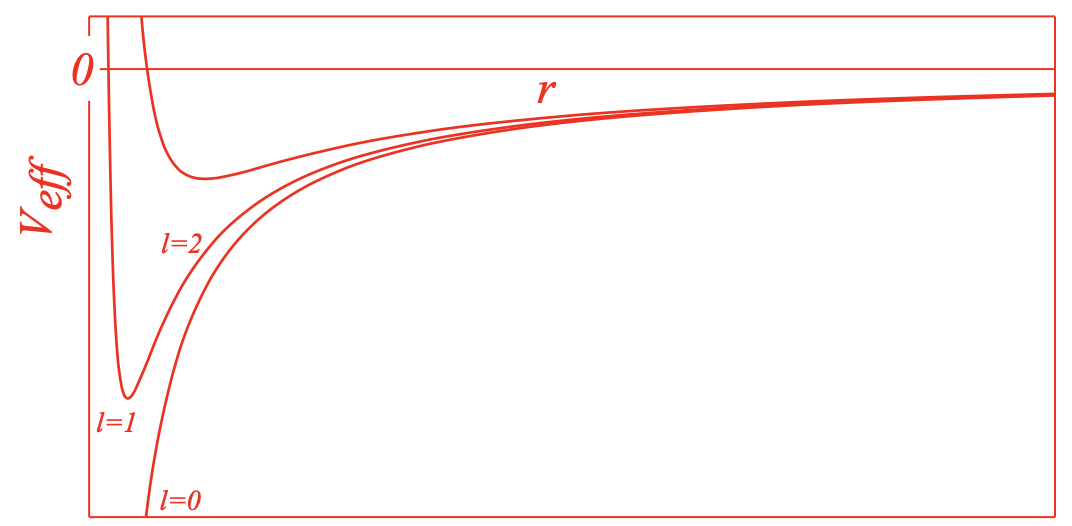
\includegraphics[width=0.5\textwidth]{fig1.png}
        \caption{Effective potential for different values of $\ell$.}
    \end{figure}

    We can note that the more negative the value of $E$ is, the less it is possible to access orbits of large $\ell$ ($\ell_{m}$ decreases). Eventually, only the $s$ orbitals are accessible ($\ell_{m} = 0$). We will see that the energy quantization we will find later reflects this aspect.

    It should be noted that, unlike classical mechanics, we will see that even in a bound state, the probability of finding the electron outside the zone is not zero because the potential well in which the electron is trapped is not infinitely deep.}

    \item Transform the differential equation on the radial wave function by introducing the function:

    $$
    u_{E, \ell}(r) = r R_{E, \ell}(r)
    $$

    then rewrite this equation using the variables $x = r \sqrt{\frac{8 \mu |E|}{\hbar^{2}}}$ and $\lambda = \frac{Z e^{2}}{4 \pi \epsilon_{0} \hbar} \sqrt{\frac{\mu}{2 |E|}}$ for the states of energy $E < 0$ (bound states).

    {\color{red}\textbf{Solution:} The bound states correspond to $E < 0$ or $E = -|E|$.

    $$
    \begin{gathered}
    \text{We have} \quad -\frac{\hbar^{2}}{2 \mu} \frac{1}{r} \frac{\partial^{2} u_{E, \ell}}{\partial r^{2}}(r) + \left(V_{\text{eff}}(r) - E\right) \frac{1}{r} u_{E, \ell}(r) = 0 \\
    \text{and thus} \quad -\frac{\hbar^{2}}{2 \mu} \frac{\partial^{2} u_{E, \ell}}{\partial r^{2}}(r) + \left(\frac{\hbar^{2} \ell(\ell+1)}{2 \mu} \frac{1}{r^{2}} - \frac{Z e^{2}}{4 \pi \epsilon_{0}} \frac{1}{r} + |E|\right) u_{E, \ell}(r) = 0
    \end{gathered}
    $$

    The change of variables $(r \rightarrow x, |E| \rightarrow \lambda)$ allows us to have a dimensionless equation:

    $$
    \frac{\partial^{2} u_{E, \ell}}{\partial r^{2}} = \left(\frac{d x}{d r}\right)^{2} \frac{\partial^{2} u_{E, \ell}}{\partial x^{2}} \Rightarrow \frac{\partial^{2} u_{E, \ell}}{\partial x^{2}}(x) - \left(\frac{\ell(\ell+1)}{x^{2}} - \frac{\lambda}{x} + \frac{1}{4}\right) u_{E, \ell}(x) = 0
    $$}

    \item Find the asymptotic solutions of this equation for $x \rightarrow \infty$ and for $x \rightarrow 0$. Deduce that the general form of the solutions can be written as:

    $$
    u_{E, \ell}(x) = e^{-x / 2} x^{\ell+1} g(x)
    $$

    {\color{red}\textbf{Solution:}

    $$
    \begin{gathered}
    x \rightarrow \infty \Rightarrow \frac{\partial^{2} u_{E, \ell}}{\partial x^{2}}(x) - \frac{1}{4} u_{E, \ell}(x) = 0 \quad \Rightarrow \quad u_{E, \ell}(x) \sim e^{-x / 2} \\
    x \rightarrow 0 \Rightarrow \frac{\partial^{2} u_{E, \ell}}{\partial x^{2}}(x) - \frac{\ell(\ell+1)}{x^{2}} u_{E, \ell}(x) = 0 \quad \Rightarrow \quad u_{E, \ell}(x) \sim x^{\ell+1}
    \end{gathered}
    $$}

    \item Determine the differential equation satisfied by the function $g(x)$. Expand the function $g(x)$ in a Taylor series and find the recurrence condition for the coefficients $c_{k}$.

    {\color{red}\textbf{Solution:} After a somewhat tedious calculation, we first arrive at:

    $$
    \begin{gathered}
    \frac{\partial^{2} u_{E, \ell}}{\partial x^{2}}(x) = e^{-x / 2} x^{\ell} \left[x \frac{\partial^{2} g(x)}{\partial x^{2}} + \frac{\partial g(x)}{\partial x}(2(\ell+1) - x) + g(x) \left(\frac{\ell(\ell+1)}{x} - (\ell+1) + \frac{x}{4}\right)\right] \\
    \text{then} \quad x \frac{\partial^{2} g(x)}{\partial x^{2}} + (2(\ell+1) - x) \frac{\partial g(x)}{\partial x} + (\lambda - (\ell+1)) g(x) = 0
    \end{gathered}
    $$

    By writing $g(x)$ in polynomial form, we have:

    $$
    \begin{gathered}
    g(x) = \sum_{k=0}^{\infty} c_{k} x^{k} \quad \text{and} \quad \frac{\partial g(x)}{\partial x} = \sum_{k=0}^{\infty} (k+1) c_{k+1} x^{k} \quad \text{and} \quad x \frac{\partial g(x)}{\partial x} = \sum_{k=1}^{\infty} k c_{k} x^{k} \\
    x \frac{\partial^{2} g(x)}{\partial x^{2}} = x \sum_{k=2}^{\infty} k(k-1) c_{k} x^{k-2} = \sum_{k=1}^{\infty} k(k+1) c_{k+1} x^{k} = \sum_{k=0}^{\infty} k(k+1) c_{k+1} x^{k} \\
    \Rightarrow \sum_{k=0}^{\infty} \left[((k+1) k + 2(\ell+1)(k+1)) c_{k+1} + (\lambda - k - \ell - 1) c_{k}\right] x^{k} = 0
    \end{gathered}
    $$

    We deduce that $\forall k, ((k+1) k + 2(\ell+1)(k+1)) c_{k+1} + (\lambda - k - \ell - 1) c_{k} = 0$.}

    \item Show that the above series must terminate at an index $k_{\max}$. Deduce that the energy levels of the bound states are indexed by a principal quantum number $n = \ell + 1 + k_{\max} \geq \ell + 1$.

    {\color{red}\textbf{Solution:} When $k$ is large, we have $k c_{k+1} \sim c_{k}$, i.e., $c_{k} \sim 1 / (k!)$. We deduce that $g(x)$ would behave like $e^{x}$ at infinity for $x$, making the function $u_{E, \ell}(x)$ divergent and thus non-physical. We deduce that $g(x)$ must be truncated.

    $$
    c_{k_{\max} + 1} = 0 \quad \Leftrightarrow \quad \lambda - k_{\max} - \ell - 1 = 0 \quad \Leftrightarrow \quad \lambda = k_{\max} + \ell + 1
    $$

    $\lambda$ is thus a strictly positive integer traditionally denoted by $n$ and which is the principal quantum number ($n$ is directly related to the energy).

    $$
    n = \frac{Z e^{2}}{4 \pi \epsilon_{0} \hbar} \sqrt{\frac{\mu}{2 \left|E_{n}\right|}} \Rightarrow E_{n} = -\frac{\mu Z^{2} e^{4}}{2 \left(4 \pi \epsilon_{0}\right)^{2} \hbar^{2}} \frac{1}{n^{2}} = -\frac{R_{y}}{n^{2}} = -\frac{Z^{2} R_{\infty}}{n^{2}}
    $$

    $R_{\infty}$ being the Rydberg constant (ionization energy of the hydrogen atom).

    To reconstruct the functions $R_{n, \ell}(r)$, we can note that $x = \frac{2 r}{n r_{0}}$ where $a_{0} = Z r_{0} = \frac{4 \pi \epsilon_{0} \hbar^{2}}{\mu e^{2}}$ is the Bohr radius.

    $$
    \begin{aligned}
    & 1 s \\
    & u_{10}(x) \propto x e^{-\frac{x}{2}} \\
    & R_{10}(r) \propto e^{-\frac{r}{r_{0}}} \\
    & 2 s \\
    & u_{20}(x) \propto \left(1 - \frac{x}{2}\right) x e^{-\frac{x}{2}} \\
    & R_{20}(r) \propto \left(1 - \frac{r}{2 r_{0}}\right) e^{-\frac{r}{2 r_{0}}} \\
    & 2 p \\
    & u_{21}(x) \propto x^{2} e^{-\frac{x}{2}} \\
    & R_{21}(r) \propto \frac{r}{r_{0}} e^{-\frac{r}{2 r_{0}}}
    \end{aligned}
    $$

    The probability density of finding the electron at $\vec{r}$ is $\mathcal{P}(\vec{r}) = \left|R_{n \ell}(r)\right|^{2} \left|Y_{\ell m}(\theta, \phi)\right|^{2}$. Given that here we are only interested in the radial aspect of things, it is more natural to define a radial probability density, $\mathcal{D}(r)$, by integrating $\mathcal{P}(\vec{r})$ over the sphere of radius $r$: $\mathcal{D}(r) = \iint \mathcal{P}(\vec{r}) r^{2} \sin \theta d \theta d \phi = 4 \pi r^{2} \left|R_{n \ell}(r)\right|^{2}$ (by construction, the integral of $\left|Y_{\ell m}(\theta, \phi)\right|^{2}$ over the sphere of radius $r$ is equal to 1). The figure below shows $\mathcal{D}(r)$ for the orbits $1s, 2s$ and $2p$.

    \begin{figure}[h]
        \centering
        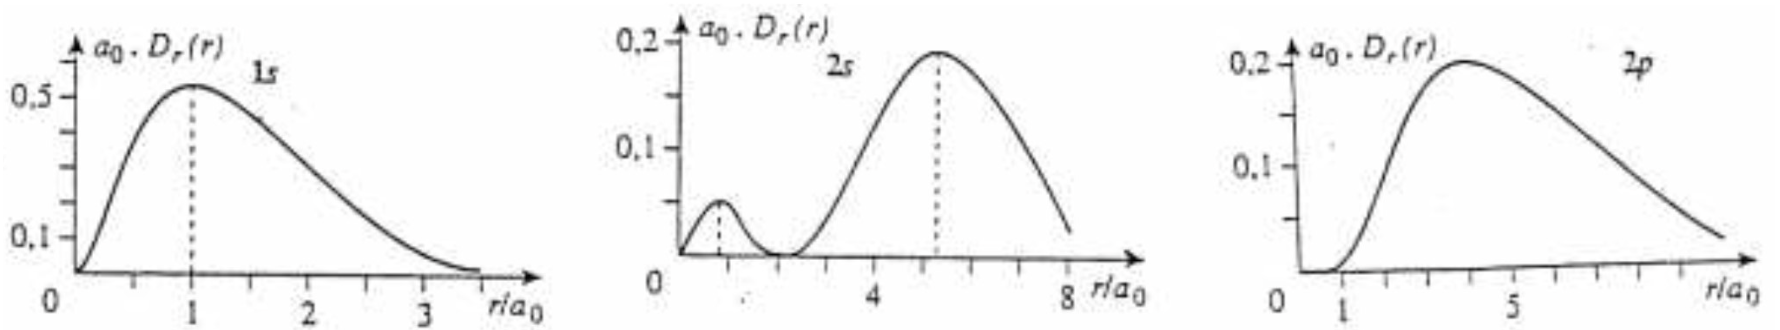
\includegraphics[width=\textwidth]{fig2.png}
        \caption{Radial probability density for different orbits.}
    \end{figure}

    We note that $\mathcal{D}(0) = 0$ even in the case of $s$ orbits, whereas $\mathcal{P}(\overrightarrow{0})$ is non-zero. We can easily generalize a few remarks:

    - $\mathcal{D}(r)$ has $n - \ell$ lobes and $n - \ell$ nodes (including the one at 0).
    - The most intense lobe is also the one farthest from the nucleus.
    - The most intense lobe is farther from the nucleus as $n$ is larger. This supports the idea that the highest energy levels ($n$ large) are those of the electrons in the outer shells (the electron is farther from the nucleus).}

    \item What would the Schrödinger equation become if we no longer assume that the nucleus is immobile?

    {\color{red}\textbf{Solution:} We must then consider the system (Nucleus $(M, \vec{r}_{1}) + \text{electron} (m, \vec{r}_{2})$) and place ourselves in the center of mass frame. By denoting $\vec{R}$ the position of the center of mass, $\mu$ the reduced mass, and $\vec{r}$ the relative position, we can show that:

    $$
    \hat{\mathcal{H}} = -\frac{\hbar^{2}}{2 M} \overrightarrow{\nabla}_{\vec{r}_{1}}^{2} - \frac{\hbar^{2}}{2 m} \overrightarrow{\nabla}_{\vec{r}_{2}}^{2} + V\left(\vec{r}_{1} - \vec{r}_{2}\right) = -\frac{\hbar^{2}}{2(M + m)} \overrightarrow{\nabla}_{\vec{R}}^{2} - \frac{\hbar^{2}}{2 \mu} \overrightarrow{\nabla_{\vec{r}}^{2}} + V(\vec{r})
    $$

    We realize that $\Psi\left(\vec{r}_{1}, \vec{r}_{2}\right)$ can be written as $\Phi(\vec{r}) \Phi^{\prime}(\vec{R})$, where $\Phi^{\prime}$ is governed by a free particle Hamiltonian (center of mass) and $\Phi$ by the Hamiltonian studied previously.}
    
\end{enumerate}

\newpage

    \section*{Series n$^{\circ} 8$: Stern \& Gerlach Experiment}

    We assume that a Stern-Gerlach apparatus consists of a preparation zone in which there is a magnetic field gradient oriented along the unit vector $\vec{u} = (\sin \theta, 0, \cos \theta)$ ($\theta$ being counted from the Oz axis). We create a beam of atoms carrying a spin $\vec{S}$ ($S = \frac{1}{2}$) in the state $|+\rangle_{\vec{u}}$, by blocking the part $|-\rangle_{\vec{u}}$ emerging from this preparation zone.

    {\color{red}\textbf{Solution:} In this series, we will place ourselves in the basis $\left\{|+\rangle_{z}, |-\rangle_{z}\right\}$ (eigenstates of $\hat{S}_{z}$). We will use:

    $$
    \hat{S}_{x} = \frac{\hbar}{2} \begin{bmatrix}
    0 & 1 \\
    1 & 0
    \end{bmatrix} = \frac{\hbar}{2} \hat{\sigma}_{x} \quad \hat{S}_{y} = \frac{\hbar}{2} \begin{bmatrix}
    0 & -i \\
    i & 0
    \end{bmatrix} = \frac{\hbar}{2} \hat{\sigma}_{y} \quad \hat{S}_{z} = \frac{\hbar}{2} \begin{bmatrix}
    1 & 0 \\
    0 & -1
    \end{bmatrix} = \frac{\hbar}{2} \hat{\sigma}_{z}
    $$}

    \begin{enumerate}
        \item Establish the expression of the matrix of the operator $\hat{S}_{\vec{u}} = \vec{u} \cdot \hat{\vec{S}}$. Diagonalize it and give the expression of the transition matrix.

        {\color{red}\textbf{Solution:} We start from $\hat{\vec{S}} = \hat{S}_{x} \overrightarrow{u_{x}} + \hat{S}_{y} \overrightarrow{u_{y}} + \hat{S}_{z} \overrightarrow{u_{z}}$ and $\vec{u} = x_{u} \overrightarrow{u_{x}} + y_{u} \overrightarrow{u_{y}} + z_{u} \overrightarrow{u_{z}}$:

        $$
        \hat{S}_{\vec{u}} = \vec{u} \cdot \hat{\vec{S}} = x_{u} \hat{S}_{x} + y_{u} \hat{S}_{y} + z_{u} \hat{S}_{z} = \sin \theta \hat{S}_{x} + \cos \theta \hat{S}_{z} = \frac{\hbar}{2} \begin{bmatrix}
        \cos \theta & \sin \theta \\
        \sin \theta & -\cos \theta
        \end{bmatrix}
        $$

        Eigenvalues of $\hat{S}_{\vec{u}}$: $\det\left[\hat{S}_{\vec{u}} - \lambda \hat{\mathcal{I}}\right] = 0 \quad \Rightarrow \quad \lambda = \pm \hbar / 2$.

        The eigenvectors of $\hat{S}_{\vec{u}}$ are defined by: $\hat{S}_{\vec{u}} |+\rangle_{\vec{u}} = \hbar / 2 |+\rangle_{\vec{u}}$ and $\hat{S}_{\vec{u}} |-\rangle_{\vec{u}} = -\hbar / 2 |-\rangle_{\vec{u}}$. By seeking $|+\rangle_{\vec{u}} = \begin{bmatrix} a \\ b \end{bmatrix}$, we must solve the system: $\begin{cases} a \cos \theta + b \sin \theta = a \\ a \sin \theta - b \cos \theta = b \end{cases}$.

        We solve $|+\rangle_{\vec{u}} = \cos \frac{\theta}{2} |+\rangle_{z} + \sin \frac{\theta}{2} |-\rangle_{z}$ and $|-\rangle_{\vec{u}} = -\sin \frac{\theta}{2} |+\rangle_{z} + \cos \frac{\theta}{2} |-\rangle_{z}$. The transition matrix $\hat{\mathcal{P}}$ from a quantization axis $z$ to an axis $\vec{u}$ can be defined by $\hat{\mathcal{P}} |+\rangle_{z} = |+\rangle_{\vec{u}}$ and $\hat{\mathcal{P}} |-\rangle_{z} = |-\rangle_{\vec{u}}$ and is written as:

        $$
        \hat{\mathcal{P}} = \begin{bmatrix}
        \cos \frac{\theta}{2} & -\sin \frac{\theta}{2} \\
        \sin \frac{\theta}{2} & \cos \frac{\theta}{2}
        \end{bmatrix} \quad \text{and} \quad \hat{\mathcal{P}}^{-1} = \begin{bmatrix}
        \cos \frac{\theta}{2} & \sin \frac{\theta}{2} \\
        -\sin \frac{\theta}{2} & \cos \frac{\theta}{2}
        \end{bmatrix} = \hat{\mathcal{P}}^{\dagger} \quad \text{(unitary)}
        $$

        We can note that $\hat{\mathcal{P}}$ has the form of a rotation matrix, but one might be surprised that the angle to be used is $\theta / 2$. In fact, it must be realized that the vector space in which $\hat{\mathcal{P}}$ acts is not that of the vectors of the $xz$ plane (in which $\vec{u}$ is) but that of the spin states.

        For example, $\theta = 2 \pi$ leads to $\hat{\mathcal{P}} = -\hat{\mathcal{I}}$ and $\hat{\mathcal{P}} |+\rangle_{z} = -|+\rangle_{z}$. We have thus rotated by $\pi$ in the space of spins, but if we interpret this result in terms of the state of the system, we see that the wave function has only changed by a phase term $(-1)$ and that therefore the spin still has complete polarization along $+z$.

        If we take $\theta = \pi$, we have $\hat{\mathcal{P}} |+\rangle_{z} = |-\rangle_{z}$ corresponding to a rotation of $\pi / 2$ in the space of spin (exchange of $|+\rangle_{z}$ and $|-\rangle_{z}$) but to an inversion of the polarization.}


    \item If we write a general state vector $|\chi\rangle = a|+\rangle_{z} + b|-\rangle_{z}$, show that the components of the average value $\langle\chi| \vec{S}|\chi\rangle$ are:

    $$
    \begin{aligned}
    \langle\chi| \hat{S}_{x}|\chi\rangle & = \hbar \Re\left(a b^{*}\right) \\
    \langle\chi| \hat{S}_{y}|\chi\rangle & = \hbar \Im\left(a^{*} b\right) \\
    \langle\chi| \hat{S}_{z}|\chi\rangle & = \hbar\left(|a|^{2} - |b|^{2}\right) / 2
    \end{aligned}
    $$

    {\color{red}\textbf{Solution:}

    $$
    \begin{aligned}
    & \left\langle\hat{S}_{x}\right\rangle = \frac{\hbar}{2}\left(a^{*}, b^{*}\right)\left[\begin{array}{cc}
    0 & 1 \\
    1 & 0
    \end{array}\right]\binom{a}{b} = \frac{\hbar}{2}\left(a^{*}, b^{*}\right)\binom{b}{a} = \frac{\hbar}{2}\left(b a^{*} + a b^{*}\right) = \hbar \Re\left(a b^{*}\right) \\
    & \left\langle\hat{S}_{y}\right\rangle = \frac{\hbar}{2}\left(a^{*}, b^{*}\right)\left[\begin{array}{cc}
    0 & -i \\
    i & 0
    \end{array}\right]\binom{a}{b} = \frac{\hbar}{2}\left(a^{*}, b^{*}\right)\binom{-i b}{i a} = i \frac{\hbar}{2}\left(a b^{*} - b a^{*}\right) = \hbar \Im\left(a^{*} b\right) \\
    & \left\langle\hat{S}_{z}\right\rangle = \frac{\hbar}{2}\left(a^{*}, b^{*}\right)\left[\begin{array}{cc}
    1 & 0 \\
    0 & -1
    \end{array}\right]\binom{a}{b} = \frac{\hbar}{2}\left(a^{*}, b^{*}\right)\binom{a}{-b} = \frac{\hbar}{2}\left(a a^{*} - b b^{*}\right)
    \end{aligned}
    $$}

    \item Establish the expression of the matrix of the rotation operator $\hat{\mathcal{R}}^{y}(\theta)$ of angle $\theta$ and axis $\vec{u}_{y}$ in the space of spins. Compare this matrix to the transition matrix obtained in 1. Determine the components of the state $|+\rangle_{\vec{a}}$ in the basis of the states $|+\rangle_{z}$ and $|-\rangle_{z}$ (eigenstates of $\hat{S}_{z}$).

    {\color{red}\textbf{Solution:} We can note that $\hat{\sigma_{y}}^{2} = \hat{\mathcal{I}}$ and thus $\forall k \in \mathbb{N} \quad \hat{\sigma_{y}}^{2 k} = \hat{\mathcal{I}}$ and $\hat{\sigma_{y}}^{2 k+1} = \hat{\sigma_{y}}$.

    $$
    \begin{gathered}
    \hat{\mathcal{R}}^{y}(\theta) = e^{-\frac{i \theta}{\hbar} \hat{S}_{x} \vec{u}_{y}} = e^{-\frac{i \theta}{\hbar} \hat{S}_{y}} = e^{-i \frac{\theta}{2} \hat{\sigma}_{y}} = \sum_{k=0}^{\infty}\left(-i \frac{\theta}{2}\right)^{k} \frac{\hat{\sigma_{y}}^{k}}{k!} \\
    \hat{\mathcal{R}}^{y}(\theta) = \sum_{k=0}^{\infty}\left[\left(-i \frac{\theta}{2}\right)^{2 k} \frac{\hat{\mathcal{I}}}{(2 k)!} + \left(-i \frac{\theta}{2}\right)^{2 k+1} \frac{\hat{\sigma_{y}}}{(2 k+1)!}\right] = \mathcal{I} \sum_{k=0}^{\infty}\left(\frac{\theta}{2}\right)^{2 k} \frac{(-1)^{k}}{(2 k)!} - i \hat{\sigma}_{y} \sum_{k=0}^{\infty}\left(\frac{\theta}{2}\right)^{2 k+1} \frac{(-1)^{k}}{(2 k+1)!} \\
    \Rightarrow \quad \hat{\mathcal{R}}^{y}(\theta) = \cos \frac{\theta}{2} \hat{\mathcal{I}} - i \sin \frac{\theta}{2} \hat{\sigma}_{y} = \left[\begin{array}{cc}
    \cos \frac{\theta}{2} & -\sin \frac{\theta}{2} \\
    \sin \frac{\theta}{2} & \cos \frac{\theta}{2}
    \end{array}\right] = \hat{\mathcal{P}}
    \end{gathered}
    $$

    We can note that $\hat{\mathcal{P}}^{\dagger}$ (or $\hat{\mathcal{P}}^{-1}$) corresponds to $\hat{\mathcal{R}}^{y}(-\theta)$ (rotation in the opposite direction). It is also interesting to see that this operator allows transforming the state vector but also the operators. We have:

    $$
    { }_{\vec{a}}\left\langle+| \hat{S}_{\vec{a}}|+\right\rangle_{\vec{a}} = { }_{z}\left\langle+| \hat{S}_{z}|+\right\rangle_{z} \quad \Rightarrow \quad \hat{S}_{\vec{a}} = \hat{\mathcal{P}} \hat{S}_{z} \hat{\mathcal{P}}^{\dagger}
    $$

    After being prepared in the state $|\chi\rangle = |+\rangle_{\vec{a}}$, the spins then pass through a region where a magnetic field $\vec{B} = B \vec{u}_{x}$ is applied. The time required for the atoms to pass through this region is $T$.}

    \item Show that during the passage through this region the state vector evolves in time according to:

    $$
    |\chi(t)\rangle = \exp \left(-i \hat{\sigma}_{x} \frac{\phi(t)}{2}\right)|\chi\rangle = \left[\hat{\mathcal{I}} \cos \left(\frac{\phi(t)}{2}\right) - i \hat{\sigma}_{x} \sin \left(\frac{\phi(t)}{2}\right)\right]|\chi\rangle
    $$

    where $\phi(t) = |\gamma| B t$ and $\gamma = q / m$ is the gyromagnetic factor.

    {\color{red}\textbf{Solution:} In this region, the Hamiltonian is written as $\hat{\mathcal{H}} = -\gamma \vec{\hat{S}} \cdot \vec{B} = \frac{\hbar |\gamma| B}{2} \hat{\sigma_{x}}$.

    Stern and Gerlach conducted their experiment on silver atoms $(Z=47)$. The electronic configuration of Ag is $(\ldots 4 d^{10} 5 s^{1})$ so that the spin to consider is that of the $5s$ electron (the only unpaired electron). This is why $\gamma < 0$ and it was chosen to write $\gamma = -|\gamma|$. The second thing to be careful about when defining the magnetic moment associated with the spin is in the definition of the spin itself. Here the spin indeed has the dimension of an angular momentum, but for some authors, for simplification, the spin is dimensionless (the $\hbar$ is removed). We then have $\vec{S} = \hbar \vec{I}$ and it is $\vec{I}$ that is called "spin".

    $$
    |\chi(t)\rangle = e^{-\frac{i}{\hbar} \hat{\mathcal{H}} t}|\chi\rangle = e^{-i \frac{\phi(t)}{2} \hat{\sigma}_{x}}|\chi\rangle = \hat{\mathcal{R}}^{x}(\phi(t))|\chi\rangle = \left[\hat{\mathcal{I}} \cos \left(\frac{\phi(t)}{2}\right) - i \hat{\sigma}_{x} \sin \left(\frac{\phi(t)}{2}\right)\right]|\chi\rangle
    $$

    We recognize that the evolution term is a rotation operator around $x$ which is expressed in the same way as that around $y$ because we also have $\hat{\sigma_{x}}^{2} = \hat{\mathcal{I}}$.

    \item What are the components of the state vector in the basis $|+\rangle_{z}, |-\rangle_{z}$ after a time $T$?

    \textbf{\textcolor{red}{Solution:}} $|\chi\rangle = a|+\rangle_{z} + b|-\rangle_{z} = |+\rangle_{\vec{\alpha}} = \cos \frac{\theta}{2}|+\rangle_{z} + \sin \frac{\theta}{2}|-\rangle_{z}$

    $$
    |\chi(T)\rangle = \left[\begin{array}{cc}
    \cos \frac{\phi(T)}{2} & -i \sin \frac{\phi(T)}{2} \\
    -i \sin \frac{\phi(T)}{2} & \cos \frac{\phi(T)}{2}
    \end{array}\right]\binom{a}{b} = \binom{\cos \frac{\phi(T)}{2} \cos \frac{\theta}{2} - i \sin \frac{\phi(T)}{2} \sin \frac{\theta}{2}}{\cos \frac{\phi(T)}{2} \sin \frac{\theta}{2} - i \sin \frac{\phi(T)}{2} \cos \frac{\theta}{2}}
    $$}

    \item Show that the probabilities of finding the spin in the states $|+\rangle_{z}$ and $|-\rangle_{z}$ are:

    $$
    \begin{aligned}
    & P_{z}(+) = 1 / 2[1 + \cos \theta \cos \phi(T)] \\
    & P_{z}(-) = 1 / 2[1 - \cos \theta \cos \phi(T)]
    \end{aligned}
    $$

    {\color{red}\textbf{Solution:}

    $$
    \begin{aligned}
    & P_{z}(+) = \left|{ }_{z}\langle+| \chi(T)\rangle\right|^{2} = \cos ^{2} \frac{\phi(T)}{2} \cos ^{2} \frac{\theta}{2} + \sin ^{2} \frac{\phi(T)}{2} \sin ^{2} \frac{\theta}{2} = \frac{1}{2}[1 + \cos \theta \cos \phi(T)] \\
    & P_{z}(-) = \left|{ }_{z}\langle-| \chi(T)\rangle\right|^{2} = \cos ^{2} \frac{\phi(T)}{2} \sin ^{2} \frac{\theta}{2} + \sin ^{2} \frac{\phi(T)}{2} \cos ^{2} \frac{\theta}{2} = \frac{1}{2}[1 - \cos \theta \cos \phi(T)]
    \end{aligned}
    $$}

    Provide a physical interpretation of this result.

    {\color{red}\textbf{Solution:} We understand (partially) that the motion of $\vec{S}$ is a precession motion. At this stage, we can only say that the component $S_{z}$ oscillates with an angular frequency $\omega_{L} = |\gamma| B$: indeed $S_{z} = \langle\vec{S}_{z}\rangle = \hbar / 2\left(P_{z}(+) - P_{z}(-)\right) = (\hbar / 2) \cos \theta \cos \phi(T)$.}

    \item Show that the components of $\langle\chi(T)| \hat{\vec{S}}|\chi(T)\rangle$ are:

    $$
    \begin{aligned}
    \langle\chi(T)| \hat{S}_{x}|\chi(T)\rangle & = \frac{\hbar}{2} \sin \theta \\
    \langle\chi(T)| \hat{S}_{y}|\chi(T)\rangle & = -\frac{\hbar}{2} \cos \theta \sin \phi(T) \\
    \langle\chi(T)| \hat{S}_{z}|\chi(T)\rangle & = \frac{\hbar}{2} \cos \theta \cos \phi(T)
    \end{aligned}
    $$

    {\color{red}\textbf{Solution:} According to the results of question 2:

    $$
    \begin{aligned}
    & \left\langle\hat{S}_{x}\right\rangle = \hbar \Re\left(\left(\cos \frac{\phi(T)}{2} \cos \frac{\theta}{2} - i \sin \frac{\phi(T)}{2} \sin \frac{\theta}{2}\right)\left(\cos \frac{\phi(T)}{2} \sin \frac{\theta}{2} + i \sin \frac{\phi(T)}{2} \cos \frac{\theta}{2}\right)\right) \\
    & = \hbar\left(\cos ^{2} \frac{\phi(T)}{2} \cos \frac{\theta}{2} \sin \frac{\theta}{2} + \sin ^{2} \frac{\phi(T)}{2} \cos \frac{\theta}{2} \sin \frac{\theta}{2}\right) = \frac{\hbar}{2} \sin \theta \\
    & \left\langle\hat{S}_{y}\right\rangle = \hbar \Im\left(\left(\cos \frac{\phi(T)}{2} \cos \frac{\theta}{2} + i \sin \frac{\phi(T)}{2} \sin \frac{\theta}{2}\right)\left(\cos \frac{\phi(T)}{2} \sin \frac{\theta}{2} - i \sin \frac{\phi(T)}{2} \cos \frac{\theta}{2}\right)\right) \\
    & = \hbar\left(\sin \frac{\phi(T)}{2} \cos \frac{\phi(T)}{2} \sin ^{2} \frac{\theta}{2} - \cos \frac{\phi(T)}{2} \sin \frac{\phi(T)}{2} \cos ^{2} \frac{\theta}{2}\right) = -\frac{\hbar}{2} \cos \theta \sin \phi(T) \\
    & \left\langle\hat{S}_{z}\right\rangle = \frac{\hbar}{2}\left(P_{z}(+) - P_{z}(-)\right) = \frac{\hbar}{2} \cos \theta \cos \phi(T)
    \end{aligned}
    $$}

    \item Describe the geometric motion as a function of $T$ of the vector whose components are the average values of $\hat{S}_{x}, \hat{S}_{y}$ and $\hat{S}_{z}$. Provide a physical interpretation. Does the quantum result differ from the classical result?

    {\color{red}\textbf{Solution:} We can note that $\left\langle\hat{S}_{x}\right\rangle$ does not depend on time. Since $||\vec{S}|| = \hbar / 2$ is constant, this means that $\vec{S}$ is on a cone with axis $Ox$ and apex angle $\pi - 2 \theta$. Then we notice that the tip of $\vec{S}$ describes a circle in the $yz$ plane. The circle is traversed in the direct sense with an angular velocity $\omega_{L} = |\gamma| B = -\gamma B$. We thus find the Larmor precession.

    The difference with the classical description lies in the expression of the gyromagnetic factor $\gamma$ which is then $\frac{q}{2 m}$. In classical mechanics, the very notion of spin does not exist, and the difference we are talking about here is rather a difference between the magnetic moment arising from the orbital moment on the one hand and from the spin on the other. When it comes to the orbital moment, it is easy to express the gyromagnetic factor using a classical model of diamagnetism (an electron with orbital moment $L$ is equivalent to a current loop which induces a magnetic moment $\mu = \frac{q}{2 m} L$). For the spin, it is more complicated, and we need to go through the Dirac equation (relativistic approach) to find that $\gamma = \frac{q}{m}$. To reconcile the two approaches, we introduce the Landé factor $(g)$:

    $$
    \gamma = g \frac{|q|}{2 m} \quad \text{with} \quad g \approx -1 (\text{orbital}) \quad \text{and} \quad g \approx -2 (\text{spin})
    $$

    We can note that the sign of the charge has been transferred to $g$.

    Finally, you frequently find in the literature for the spin magnetic moment of the electron the following expression:

    $$
    \vec{\mu} = g \mu_{B} \vec{S} \quad \text{with} \quad \mu_{B} = \frac{e \hbar}{2 m}
    $$

    This form assumes that the spin has been divided by $\hbar$ (dimensionless spin).

    $\mu_{B}$ is the Bohr magneton. It is also called the "magnetic quantum" because it corresponds to the amplitude of the spin magnetic moment of the electron.}
    
    \newpage
    \end{enumerate}

    \section*{Series n$^{\circ} 9$: Combination of Spins}

    Exercise: Let the orbital angular momentum operator $\hat{\vec{L}} = \hat{\vec{r}} \times \hat{\vec{p}}$. Calculate the following commutators:

    $$
    \left[\hat{L}_{\alpha}, \hat{r}_{\beta}\right], \quad \left[\hat{L}_{\alpha}, \hat{p}_{\beta}\right], \quad \left[\hat{L}_{\alpha}, \hat{L}_{\beta}\right]
    $$

    where the indices $\alpha$ and $\beta$ each denote any one of the components along $x, y$ or $z$.

    {\color{red}\textbf{Solution:} Using the classical relations: $\left[\hat{r}_{\alpha}, \hat{r}_{\beta}\right] = 0, \quad \left[\hat{p}_{\alpha}, \hat{p}_{\beta}\right] = 0, \quad \left[\hat{r}_{\alpha}, \hat{p}_{\beta}\right] = i \hbar \delta_{\alpha \beta}$, we show ($\alpha, \beta, \gamma$ taken in the direct sense):

    $$
    \hat{L}_{\gamma} = \hat{r}_{\alpha} \hat{p}_{\beta} - \hat{r}_{\beta} \hat{p}_{\alpha}
    $$

    $$
    \left[\hat{L}_{\alpha}, \hat{r}_{\alpha}\right] = 0, \quad \left[\hat{L}_{\alpha}, \hat{r}_{\beta}\right] = i \hbar \hat{r}_{\gamma}, \quad \left[\hat{L}_{\alpha}, \hat{p}_{\alpha}\right] = 0, \quad \left[\hat{L}_{\alpha}, \hat{p}_{\beta}\right] = i \hbar \hat{p}_{\gamma}, \quad \left[\hat{L}_{\alpha}, \hat{L}_{\alpha}\right] = 0, \quad \left[\hat{L}_{\alpha}, \hat{L}_{\beta}\right] = i \hbar \hat{L}_{\gamma}
    $$}
    

    We consider two spins $\frac{1}{2}$ which can be, for example, the spins of the two electrons of a Helium atom. We seek to characterize the behavior of the total spin of the atom. Each spin is represented by a state vector $\left|\phi_{i}\right\rangle$ in a Hilbert space of dimension 2. We denote $\vec{S}_{i}$ the vector operator of each spin. We introduce $|\uparrow\rangle_{i}$ and $|\downarrow\rangle_{i}$ the eigenstates of the operator $\hat{S}_{z, i}$.

    \begin{enumerate}
        \item Construction of the "total spin".

        \begin{enumerate}
            \item From the states $\left|\phi_{1}\right\rangle$ and $\left|\phi_{2}\right\rangle$, write a general state of the total system consisting of spins 1 and 2. Give a basis of the resulting vector space, as well as its dimension.

            {\color{red}\textbf{Solution:} $\left|\phi_{i}\right\rangle = a_{i}|\uparrow\rangle_{i} + b_{i}|\downarrow\rangle_{i}$ vector of $\mathcal{E}_{i}$ (dimension 2).

            $$
            |\phi\rangle = \left|\phi_{1}\right\rangle \otimes \left|\phi_{2}\right\rangle = a_{1} a_{2}|\uparrow\rangle_{1} \otimes |\uparrow\rangle_{2} + a_{1} b_{2}|\uparrow\rangle_{1} \otimes |\downarrow\rangle_{2} + a_{2} b_{1}|\downarrow\rangle_{1} \otimes |\uparrow\rangle_{2} + b_{1} b_{2}|\downarrow\rangle_{1} \otimes |\downarrow\rangle_{2}
            $$

            $\left\{|\uparrow\rangle_{1} \otimes |\uparrow\rangle_{2}, |\uparrow\rangle_{1} \otimes |\downarrow\rangle_{2}, |\downarrow\rangle_{1} \otimes |\uparrow\rangle_{2}, |\downarrow\rangle_{1} \otimes |\downarrow\rangle_{2}\right\}$ is denoted $\left\{|\uparrow \uparrow\rangle, |\uparrow \downarrow\rangle, |\downarrow \uparrow\rangle, |\downarrow \downarrow\rangle\right\}$ constitutes a basis of the product space $\mathcal{E} = \mathcal{E}_{1} \otimes \mathcal{E}_{2}$ (dimension 4).

            Show that the states of this product basis are eigenstates of $\hat{S}_{1}^{2}, \hat{S}_{2}^{2}, \hat{S}_{z, 1}$ and $\hat{S}_{z, 2}$ and give their eigenvalues. Specify on which subspaces of the state space these operators act.

            \textbf{Solution:} In general, we can denote a vector of this product basis $\left|S_{1} m_{1}, S_{2} m_{2}\right\rangle$. In this exercise $S_{1} = S_{2} = 1 / 2$.

            $$
            \begin{aligned}
            \hat{S}_{z, 1}\left|S_{1} m_{1}, S_{2} m_{2}\right\rangle & = \hbar m_{1}\left|S_{1} m_{1}, S_{2} m_{2}\right\rangle \\
            \hat{S}_{z, 2}\left|S_{1} m_{1}, S_{2} m_{2}\right\rangle & = \hbar m_{2}\left|S_{1} m_{1}, S_{2} m_{2}\right\rangle \\
            \hat{S}_{1}^{2}\left|S_{1} m_{1}, S_{2} m_{2}\right\rangle & = \hbar^{2} S_{1}\left(S_{1} + 1\right)\left|S_{1} m_{1}, S_{2} m_{2}\right\rangle = \frac{3}{4} \hbar^{2}\left|S_{1} m_{1}, S_{2} m_{2}\right\rangle \\
            \hat{S}_{2}^{2}\left|S_{1} m_{1}, S_{2} m_{2}\right\rangle & = \hbar^{2} S_{2}\left(S_{2} + 1\right)\left|S_{1} m_{1}, S_{2} m_{2}\right\rangle = \frac{3}{4} \hbar^{2}\left|S_{1} m_{1}, S_{2} m_{2}\right\rangle
            \end{aligned}
            $$


All of this can be understood from a matrix perspective (the matrices are diagonal):

\[
\begin{aligned}
& \hat{S}_{z, 1} = \frac{\hbar}{2} \left[\begin{array}{cc}
1 & 0 \\
0 & -1
\end{array}\right] \otimes \left[\begin{array}{cc}
1 & 0 \\
0 & 1
\end{array}\right] = \frac{\hbar}{2} \left[\begin{array}{cccc}
1 & 0 & 0 & 0 \\
0 & 1 & 0 & 0 \\
0 & 0 & -1 & 0 \\
0 & 0 & 0 & -1
\end{array}\right] \\
& \hat{S}_{z, 2} = \left[\begin{array}{cc}
1 & 0 \\
0 & 1
\end{array}\right] \otimes \frac{\hbar}{2} \left[\begin{array}{cc}
1 & 0 \\
0 & -1
\end{array}\right] = \frac{\hbar}{2} \left[\begin{array}{cccc}
1 & 0 & 0 & 0 \\
0 & -1 & 0 & 0 \\
0 & 0 & 1 & 0 \\
0 & 0 & 0 & -1
\end{array}\right] \\
& \hat{S}_{1}^{2} = \hat{S}_{2}^{2} = \frac{3 \hbar^{2}}{4} \left[\begin{array}{ll}
1 & 0 \\
0 & 1
\end{array}\right] \otimes \left[\begin{array}{ll}
1 & 0 \\
0 & 1
\end{array}\right] = \frac{3 \hbar^{2}}{4} \left[\begin{array}{cccc}
1 & 0 & 0 & 0 \\
0 & 1 & 0 & 0 \\
0 & 0 & 1 & 0 \\
0 & 0 & 0 & 1
\end{array}\right]
\end{aligned}
\]

The calculation of the tensor product of two matrices follows these rules:

\[
\left[\begin{array}{ll}
a & b \\
c & d
\end{array}\right] \otimes \left[\begin{array}{cc}
A & B \\
C & D
\end{array}\right] = \left[\begin{array}{cccc}
a A & a B & b A & b B \\
a C & a D & b C & b D \\
c A & c B & d A & d B \\
c C & c D & d C & d D
\end{array}\right]
\]}


    \item We define the total spin operator \(\hat{\vec{S}} = \hat{\vec{S}}_{1} \otimes \hat{\mathcal{I}} + \hat{\mathcal{I}} \otimes \hat{\vec{S}}_{2}\), where \(\hat{\mathcal{I}}\) represents the identity. Explain this notation. On which space does \(\hat{\vec{S}}\) act?

    {\color{red}\textbf{Solution:} To be able to sum two operators that do not act on the same space, it is necessary to embed them in a common space \(\mathcal{E} = \mathcal{E}_{1} \otimes \mathcal{E}_{2}\). \(\hat{\vec{S}}_{1}\) is written as \(\hat{\vec{S}}_{1} \otimes \hat{\mathcal{I}}\) because it only acts in \(\mathcal{E}_{1}\). Similarly, \(\hat{\vec{S}}_{2}\) is written as \(\hat{\mathcal{I}} \otimes \hat{\vec{S}}_{2}\) because it only acts in \(\mathcal{E}_{2}\).

    Recall the commutation relations that the components of \(\hat{\vec{S}}\) must satisfy.

    \textbf{Solution:} The components of \(\hat{\vec{S}}\) are the sums of the components of \(\hat{\vec{S}}_{1}\) and \(\hat{\vec{S}}_{2}\). They therefore obey the same commutation rules:

    \[
    \left[\hat{S}_{\alpha}, \hat{S}_{\alpha}\right] = 0 \quad \text{and} \quad \left[\hat{S}_{\alpha}, \hat{S}_{\beta}\right] = i \hbar \hat{S}_{\gamma} \quad (\alpha, \beta, \gamma) \text{ direct}
    \]

    Show that the four operators \(\hat{S}^{2}, \hat{S}_{z}, \hat{S}_{1}^{2}\) and \(\hat{S}_{2}^{2}\) commute with each other and consequently are diagonalizable in the same basis.

    \textbf{Solution:} \(-\hat{S}_{z} = \hat{S}_{1 z} + \hat{S}_{2 z}\) thus commutes with \(\hat{S}_{1}^{2}\) and \(\hat{S}_{2}^{2}\).

    \[
    -\hat{S}^{2} = \hat{S}_{x}^{2} + \hat{S}_{y}^{2} + \hat{S}_{z}^{2} \quad \text{so} \quad \left[\hat{S}^{2}, \hat{S}_{z}\right] = \left[\hat{S}_{x}^{2}, \hat{S}_{z}\right] + \left[\hat{S}_{y}^{2}, \hat{S}_{z}\right] + \left[\hat{S}_{z}^{2}, \hat{S}_{z}\right] = \left[\hat{S}_{x}^{2}, \hat{S}_{z}\right] + \left[\hat{S}_{y}^{2}, \hat{S}_{z}\right]
    \]

    \[
    \left[\hat{S}^{2}, \hat{S}_{z}\right] = \hat{S}_{x} \left[\hat{S}_{x}, \hat{S}_{z}\right] + \left[\hat{S}_{x}, \hat{S}_{z}\right] \hat{S}_{x} + \hat{S}_{y} \left[\hat{S}_{y}, \hat{S}_{z}\right] + \left[\hat{S}_{y}, \hat{S}_{z}\right] \hat{S}_{y} = 0
    \]

    \(-\hat{S}^{2} = \hat{\vec{S}}^{2} = \hat{S}_{1}^{2} + \hat{S}_{2}^{2} + 2 \hat{\vec{S}}_{1} \cdot \hat{\vec{S}}_{2}\) (since \(\hat{\vec{S}}_{1}\) and \(\hat{\vec{S}}_{2}\) commute). Therefore, \(\hat{S}^{2}\) commutes with \(\hat{S}_{1}^{2}\) and \(\hat{S}_{2}^{2}\).}

    \item Verify that \(\hat{S}^{2}\) does not commute with \(\hat{S}_{z, 1}\) and \(\hat{S}_{z, 2}\). Conclude that the previously defined product basis is not a common eigenbasis for \(\hat{S}^{2}, \hat{S}_{z}, \hat{S}_{1}^{2}\) and \(\hat{S}_{2}^{2}\).

    {\color{red}\textbf{Solution:}

    \[
    \begin{aligned}
    \left[\hat{S}^{2}, \hat{S}_{z, 1}\right] & = \left[\hat{S}_{1}^{2}, \hat{S}_{z, 1}\right] + \left[\hat{S}_{2}^{2}, \hat{S}_{z, 1}\right] + \left[2 \hat{\vec{S}}_{1} \cdot \hat{\vec{S}}_{2}, \hat{S}_{z, 1}\right] = 2 \left[\hat{\vec{S}}_{1} \cdot \hat{\vec{S}}_{2}, \hat{S}_{z, 1}\right] \\
    & = 2 \left(\left[\hat{S}_{x, 1} \hat{S}_{x, 2}, \hat{S}_{z, 1}\right] + \left[\hat{S}_{y, 1} \hat{S}_{y, 2}, \hat{S}_{z, 1}\right] + \left[\hat{S}_{z, 1} \hat{S}_{z, 2}, \hat{S}_{z, 1}\right]\right) \\
    & = 2 i \hbar \left(-\hat{S}_{x, 2} \hat{S}_{y, 1} + \hat{S}_{y, 2} \hat{S}_{x, 1}\right) \neq 0
    \end{aligned}
    \]

    And similarly for \(\left[\hat{S}^{2}, \hat{S}_{z, 2}\right]\).}
    
    \end{enumerate}

    \item We will now seek the common eigenstates of these four operators to obtain a basis adapted to the total spin of the system.

    \begin{enumerate}
        \item Show that the states of the product basis are eigenstates of \(\hat{S}_{z}\). Give its eigenvalues and represent the matrix in this basis.

        {\color{red}\textbf{Solution:} $S_{z} \left|S_{1} m_{1}, S_{2} m_{2}\right\rangle = \left(S_{z, 1} + S_{z, 2}\right) \left|S_{1} m_{1}, S_{2} m_{2}\right\rangle = \hbar \left(m_{1} + m_{2}\right) \left|S_{1} m_{1}, S_{2} m_{2}\right\rangle\). We find this from a matrix perspective:

        \[
        \hat{S}_{z} = \frac{\hbar}{2} \left[\begin{array}{cccc}
        1 & 0 & 0 & 0 \\
        0 & 1 & 0 & 0 \\
        0 & 0 & -1 & 0 \\
        0 & 0 & 0 & -1
        \end{array}\right] + \frac{\hbar}{2} \left[\begin{array}{cccc}
        1 & 0 & 0 & 0 \\
        0 & -1 & 0 & 0 \\
        0 & 0 & 1 & 0 \\
        0 & 0 & 0 & -1
        \end{array}\right] = \hbar \left[\begin{array}{cccc}
        1 & 0 & 0 & 0 \\
        0 & 0 & 0 & 0 \\
        0 & 0 & 0 & 0 \\
        0 & 0 & 0 & -1
        \end{array}\right]
        \]}

        \item Recall the action of the operators \(\hat{S}_{x, i}, \hat{S}_{y, i}\) and \(\hat{S}_{z, i}\) on the states \(|\uparrow\rangle_{i}\) and \(|\downarrow\rangle_{i}\). Calculate the matrix elements of the operator \(\hat{S}^{2}\) on the product basis and verify that the matrix is not diagonal.

        {\color{red}\textbf{Solution:}

        \[
        \begin{aligned}
        & \hat{S}_{x} = \frac{\hbar}{2} \left[\begin{array}{llll}
        0 & 0 & 1 & 0 \\
        0 & 0 & 0 & 1 \\
        1 & 0 & 0 & 0 \\
        0 & 1 & 0 & 0
        \end{array}\right] + \frac{\hbar}{2} \left[\begin{array}{llll}
        0 & 1 & 0 & 0 \\
        1 & 0 & 0 & 0 \\
        0 & 0 & 0 & 1 \\
        0 & 0 & 1 & 0
        \end{array}\right] = \frac{\hbar}{2} \left[\begin{array}{llll}
        0 & 1 & 1 & 0 \\
        1 & 0 & 0 & 1 \\
        1 & 0 & 0 & 1 \\
        0 & 1 & 1 & 0
        \end{array}\right] \\
        & \hat{S}_{y} = \frac{\hbar}{2} \left[\begin{array}{llll}
        0 & 0 & -i & 0 \\
        0 & 0 & 0 & -i \\
        i & 0 & 0 & 0 \\
        0 & i & 0 & 0
        \end{array}\right] + \frac{\hbar}{2} \left[\begin{array}{llll}
        0 & -i & 0 & 0 \\
        i & 0 & 0 & 0 \\
        0 & 0 & 0 & -i \\
        0 & 0 & i & 0
        \end{array}\right] = \frac{\hbar}{2} \left[\begin{array}{llll}
        0 & -i & -i & 0 \\
        i & 0 & 0 & -i \\
        i & 0 & 0 & -i \\
        0 & i & i & 0
        \end{array}\right] \\
        & \hat{S}_{z} = \frac{\hbar}{2} \left[\begin{array}{llll}
        1 & 0 & 0 & 0 \\
        0 & 1 & 0 & 0 \\
        0 & 0 & -1 & 0 \\
        0 & 0 & 0 & -1
        \end{array}\right] + \frac{\hbar}{2} \left[\begin{array}{llll}
        1 & 0 & 0 & 0 \\
        0 & -1 & 0 & 0 \\
        0 & 0 & 1 & 0 \\
        0 & 0 & 0 & -1
        \end{array}\right] = \hbar \left[\begin{array}{llll}
        1 & 0 & 0 & 0 \\
        0 & 0 & 0 & 0 \\
        0 & 0 & 0 & 0 \\
        0 & 0 & 0 & -1
        \end{array}\right]
        \end{aligned}
        \]

        \[
        \hat{S}^{2} = \hat{S}_{x}^{2} + \hat{S}_{y}^{2} + \hat{S}_{z}^{2} = \hbar^{2} \left[\begin{array}{llll}
        2 & 0 & 0 & 0 \\
        0 & 1 & 1 & 0 \\
        0 & 1 & 1 & 0 \\
        0 & 0 & 0 & 2
        \end{array}\right]
        \]

        The matrix is not diagonal, which expresses that the product basis is not an eigenbasis of \(\hat{S}^{2}\).

        Determine its eigenvalues and eigenvectors.

        \textbf{Solution:} $|\uparrow \uparrow\rangle$ and $|\downarrow \downarrow\rangle$ are still eigenvectors, and it suffices to diagonalize in the subspace $\{|\uparrow \downarrow\rangle, |\downarrow \uparrow\rangle\}$.

        \[
        \left|\begin{array}{cc}
        \hbar^{2} - \lambda & \hbar^{2} \\
        \hbar^{2} & \hbar^{2} - \lambda
        \end{array}\right| = 0 \quad \Rightarrow \quad \lambda = 0 \quad \text{or} \quad \lambda = 2 \hbar^{2}
        \]

        The associated eigenvectors are:

        \[
        |s\rangle = \frac{1}{\sqrt{2}} (|\uparrow \downarrow\rangle - |\downarrow \uparrow\rangle) \quad (\lambda = 0) \quad \left|t^{\circ}\right\rangle = \frac{1}{\sqrt{2}} (|\uparrow \downarrow\rangle + |\downarrow \uparrow\rangle) \quad (\lambda = 2 \hbar^{2})
        \]}

        \item Divide the vector space according to the eigenvalues of \(\hat{S}^{2}\). Show that this division gives two subspaces, one three-dimensional (triplet) and the other one-dimensional (singlet).

        {\color{red}\textbf{Solution:} \(\hat{S}^{2}\) has 0 as an eigenvalue associated with the vector \(|s\rangle\) which underlies a one-dimensional vector space (singlet) and \(2 \hbar^{2}\) three times degenerate associated with the vectors \(|\uparrow \uparrow\rangle\) (we will denote it \(\left|t^{+}\right\rangle\)), \(\left|t^{\circ}\right\rangle\) and \(|\downarrow \downarrow\rangle\) (we will denote it \(\left|t^{-}\right\rangle\)) which underlie a three-dimensional vector space (triplet).

        In the following, we will write the operators in the basis \(\left\{|s\rangle, \left|t^{+}\right\rangle, \left|t^{\circ}\right\rangle, \left|t^{-}\right\rangle\right\}\). We will see that the division of the vector space exposed above corresponds to the fact that the composite spin can take the appearance of a zero spin (singlet) or that of a spin 1 (triplet). Another common way to denote the eigenvectors is \(|S, m_{S}\rangle\) with \(S = 0\) or \(S = 1\). The basis is then denoted: \(\{|0, 0\rangle, |1, 1\rangle, |1, 0\rangle, |1, -1\rangle\}\).

        Determine the matrices representing \(\hat{S}_{z}, \hat{S}_{x}\) and \(\hat{S}_{y}\) in this eigenbasis of \(\hat{S}^{2}\), separating the triplet subspace and the singlet subspace.

        \textbf{Solution:} In the subspace \(\left\{\left|t^{+}\right\rangle, \left|t^{\circ}\right\rangle, \left|t^{-}\right\rangle\right\}\):

        \[
        \hat{S}_{x} = \frac{\hbar}{\sqrt{2}} \left[\begin{array}{ccc}
        0 & 1 & 0 \\
        1 & 0 & 1 \\
        0 & 1 & 0
        \end{array}\right] \quad \hat{S}_{y} = \frac{\hbar}{\sqrt{2}} \left[\begin{array}{ccc}
        0 & -i & 0 \\
        i & 0 & -i \\
        0 & i & 0
        \end{array}\right] \quad \hat{S}_{z} = \hbar \left[\begin{array}{ccc}
        1 & 0 & 0 \\
        0 & 0 & 0 \\
        0 & 0 & -1
        \end{array}\right]
        \]

        If we add to this the fact that \(\hat{S}^{2} = 2 \hbar^{2} \mathcal{I}\), we indeed have the characteristics of a spin 1 in this subspace.

        In the basis \(\left\{|s\rangle, \left|t^{+}\right\rangle, \left|t^{\circ}\right\rangle, \left|t^{-}\right\rangle\right\}\) (we will mark with a \(\sharp\) the operators to specify that they are written in this basis):

        \[
        \stackrel{\sharp S_{x}}{\sim} = \hbar \left[\begin{array}{cccc}
        0 & 0 & 0 & 0 \\
        0 & 0 & \frac{1}{\sqrt{2}} & 0 \\
        0 & \frac{1}{\sqrt{2}} & 0 & \frac{1}{\sqrt{2}} \\
        0 & 0 & \frac{1}{\sqrt{2}} & 0
        \end{array}\right] \quad \stackrel{\sharp S_{y}}{\sim} = \hbar \left[\begin{array}{cccc}
        0 & 0 & 0 & 0 \\
        0 & 0 & \frac{-i}{\sqrt{2}} & 0 \\
        0 & \frac{i}{\sqrt{2}} & 0 & \frac{-i}{\sqrt{2}} \\
        0 & 0 & \frac{i}{\sqrt{2}} & 0
        \end{array}\right] \quad \stackrel{\sharp S_{z}}{\sim} = \hbar \left[\begin{array}{cccc}
        0 & 0 & 0 & 0 \\
        0 & 1 & 0 & 0 \\
        0 & 0 & 0 & 0 \\
        0 & 0 & 0 & -1
        \end{array}\right]
        \]

        All of the above could have been obtained using the transition matrix from one basis to another:

        \[
        \begin{aligned}
        & \left\{|\uparrow \uparrow\rangle, |\uparrow \downarrow\rangle, |\downarrow \uparrow\rangle, |\downarrow \downarrow\rangle\right\} \quad \xrightarrow{\hat{\mathcal{P}}} \quad \left\{|s\rangle, \left|t^{+}\right\rangle, \left|t^{\circ}\right\rangle, \left|t^{-}\right\rangle\right\} \quad \text{we have:} \\
        & \hat{\mathcal{P}} = \left[\begin{array}{cccc}
        0 & \frac{1}{\sqrt{2}} & -\frac{1}{\sqrt{2}} & 0 \\
        1 & 0 & 0 & 0 \\
        0 & \frac{1}{\sqrt{2}} & \frac{1}{\sqrt{2}} & 0 \\
        0 & 0 & 0 & 1
        \end{array}\right] \quad \text{and} \quad \hat{\mathcal{P}}^{-1} = \hat{\mathcal{P}}^{\dagger} = \left[\begin{array}{cccc}
        0 & 1 & 0 & 0 \\
        \frac{1}{\sqrt{2}} & 0 & \frac{1}{\sqrt{2}} & 0 \\
        -\frac{1}{\sqrt{2}} & 0 & \frac{1}{\sqrt{2}} & 0 \\
        0 & 0 & 0 & 1
        \end{array}\right]
        \end{aligned}
        \]

        We can note that the columns of \(\hat{\mathcal{P}}^{\dagger}\) represent the vectors of the new basis expressed in the old one, and those of \(\hat{\mathcal{P}}\) the vectors of the old basis in the new one. We then easily verify (product of three \(4 \times 4\) matrices!) that:

        \[
        \stackrel{\sharp S_{x}}{\sim} = \hat{\mathcal{P}} \hat{S}_{x} \hat{\mathcal{P}}^{\dagger} \quad \stackrel{\sharp S_{y}}{\sim} = \hat{\mathcal{P}} \hat{S}_{y} \hat{\mathcal{P}}^{\dagger} \quad \stackrel{\sharp S_{z}}{\sim} = \hat{\mathcal{P}} \hat{S}_{z} \hat{\mathcal{P}}^{\dagger}
        \]}
        
        \end{enumerate}

        \item (Optional) We now perform a rotation of an angle \(\theta\) around the \(y\) axis. The states of each spin \(\frac{1}{2}\) then transform into \(\left|\phi_{i}^{\prime}\right\rangle = \hat{D}_{i} \left|\phi_{i}\right\rangle\) thanks to the rotation operator:

        \[
        \hat{D}_{i}(\theta, y) = \exp \left(-i \frac{\hat{S}_{y, i}}{\hbar} \theta\right) = \hat{\mathcal{I}} \cos (\theta / 2) - i \hat{\sigma}_{y} \sin (\theta / 2)
        \]

        \begin{enumerate}
            \item Determine the expression of the operator \(\hat{D}(\theta, y) = \hat{D}_{1}(\theta, y) \otimes \hat{D}_{2}(\theta, y)\) in matrix form in the product basis, then in the eigenbasis of \(\hat{S}^{2}\). Note that the singlet state remains unchanged by this rotation and that the triplet states mix among themselves but not with the singlet state.

            {\color{red}\textbf{Solution:} Let \(c = \cos (\theta / 2)\) and \(s = \sin (\theta / 2)\).

            In the product basis:

            \[
            \begin{aligned}
            & \hat{D}_{1}(\theta, y) = c \left[\begin{array}{cccc}
            1 & 0 & 0 & 0 \\
            0 & 1 & 0 & 0 \\
            0 & 0 & 1 & 0 \\
            0 & 0 & 0 & 1
            \end{array}\right] - i s \left[\begin{array}{cccc}
            0 & 0 & -i & 0 \\
            0 & 0 & 0 & -i \\
            i & 0 & 0 & 0 \\
            0 & i & 0 & 0
            \end{array}\right] = \left[\begin{array}{cccc}
            c & 0 & -s & 0 \\
            0 & c & 0 & -s \\
            s & 0 & c & 0 \\
            0 & s & 0 & c
            \end{array}\right] \\
            & \hat{D}_{2}(\theta, y) = c \left[\begin{array}{cccc}
            1 & 0 & 0 & 0 \\
            0 & 1 & 0 & 0 \\
            0 & 0 & 1 & 0 \\
            0 & 0 & 0 & 1
            \end{array}\right] - i s \left[\begin{array}{cccc}
            0 & -i & 0 & 0 \\
            i & 0 & 0 & 0 \\
            0 & 0 & 0 & -i \\
            0 & 0 & i & 0
            \end{array}\right] = \left[\begin{array}{cccc}
            c & -s & 0 & 0 \\
            s & c & 0 & 0 \\
            0 & 0 & c & -s \\
            0 & 0 & s & c
            \end{array}\right]
            \end{aligned}
            \]

            \[
            \hat{D}(\theta, y) = \left[\begin{array}{cccc}
            c & 0 & -s & 0 \\
            0 & c & 0 & -s \\
            s & 0 & c & 0 \\
            0 & s & 0 & c
            \end{array}\right] \left[\begin{array}{cccc}
            c & -s & 0 & 0 \\
            s & c & 0 & 0 \\
            0 & 0 & c & -s \\
            0 & 0 & s & c
            \end{array}\right] = \left[\begin{array}{cccc}
            c^{2} & -c s & -c s & s^{2} \\
            c s & c^{2} & -s^{2} & -c s \\
            c s & -s^{2} & c^{2} & -c s \\
            s^{2} & c s & c s & c^{2}
            \end{array}\right]
            \]

            It should be noted that it was also possible to keep \(\hat{D}_{1}(\theta, y)\) and \(\hat{D}_{2}(\theta, y)\) in their respective vector spaces of action and to write the tensor product of their matrices. We would obviously have the same result:

            \[
            \hat{D}(\theta, y) = \left[\begin{array}{cc}
            c & -s \\
            s & c
            \end{array}\right] \otimes \left[\begin{array}{cc}
            c & -s \\
            s & c
            \end{array}\right] = \left[\begin{array}{cccc}
            c^{2} & -c s & -c s & s^{2} \\
            c s & c^{2} & -s^{2} & -c s \\
            c s & -s^{2} & c^{2} & -c s \\
            s^{2} & c s & c s & c^{2}
            \end{array}\right]
            \]

            In the basis \(\left\{|s\rangle, \left|t^{+}\right\rangle, \left|t^{\circ}\right\rangle, \left|t^{-}\right\rangle\right\}\), we do not know the matrices \(\hat{\sigma}_{y, 1}\) and \(\hat{\sigma}_{y, 2}\). It is better to calculate the action of \(\hat{D}\) on the vectors. We obtain:

            \[
            \begin{aligned}
            \hat{D}(\theta, y) |s\rangle & = |s\rangle \\
            \hat{D}(\theta, y) \left|t^{+}\right\rangle & = c^{2} \left|t^{+}\right\rangle + \sqrt{2} c s \left|t^{\circ}\right\rangle + s^{2} \left|t^{-}\right\rangle \\
            \hat{D}(\theta, y) \left|t^{\circ}\right\rangle & = -\sqrt{2} c s \left|t^{+}\right\rangle + \left(c^{2} - s^{2}\right) \left|t^{\circ}\right\rangle + \sqrt{2} c s \left|t^{-}\right\rangle \\
            \hat{D}(\theta, y) \left|t^{-}\right\rangle & = s^{2} \left|t^{+}\right\rangle - \sqrt{2} c s \left|t^{\circ}\right\rangle + c^{2} \left|t^{-}\right\rangle
            \end{aligned}
            \]

            And thus in the basis \(\left\{|s\rangle, \left|t^{+}\right\rangle, \left|t^{\circ}\right\rangle, \left|t^{-}\right\rangle\right\}\):

            \[
            { }^{\sharp} \hat{D}(\theta, y) = \left[\begin{array}{cccc}
            1 & 0 & 0 & 0 \\
            0 & c^{2} & -\sqrt{2} c s & s^{2} \\
            0 & \sqrt{2} c s & \left(c^{2} - s^{2}\right) & -\sqrt{2} c s \\
            0 & s^{2} & \sqrt{2} c s & c^{2}
            \end{array}\right]
            \]

            The singlet state is indeed invariant and isolated from the triplets by the rotation. Here again, we could have used the transition matrix (now that it is established) and done the calculation (a bit tedious):

            \[
            { }^{\sharp} \hat{D}(\theta, y) = \hat{\mathcal{P}} \hat{D}(\theta, y) \hat{\mathcal{P}}^{\dagger}
            \]

            Finally:

            \[
            { }^{\sharp} \hat{D}(\theta, y) = \left[\begin{array}{cccc}
            1 & 0 & 0 & 0 \\
            0 & \frac{1 + \cos \theta}{2} & -\frac{\sin \theta}{\sqrt{2}} & \frac{1 - \cos \theta}{2} \\
            0 & \frac{\sin \theta}{\sqrt{2}} & \cos \theta & -\frac{\sin \theta}{\sqrt{2}} \\
            0 & \frac{1 - \cos \theta}{2} & \frac{\sin \theta}{\sqrt{2}} & \frac{1 + \cos \theta}{2}
            \end{array}\right]
            \]}

            \item We introduce the matrix \(\hat{\Sigma}_{y}\) of dimension 3 such that \(\hat{S}_{y} = \hbar \hat{\Sigma}_{y}\) on the triplet subspace. Calculate first \(\hat{\Sigma}_{y}^{2}\) and \(\hat{\Sigma}_{y}^{3}\), then show successively that \(\hat{D}(\theta, y)\) can be written as:

            \[
            \hat{D}(\theta, y) = \hat{\mathcal{I}} + \hat{\Sigma}_{y}^{2} (\cos \theta - 1) - i \hat{\Sigma}_{y} \sin \theta \quad \text{then} \quad \hat{D}(\theta, y) = \exp \left(-i \frac{\hat{S}_{y}}{\hbar} \theta\right)
            \]

            Compare to equation (1) and conclude on the general expression of the rotation operators.

            {\color{red}\textbf{Solution:} In the subspace \(\left\{\left|t^{+}\right\rangle, \left|t^{\circ}\right\rangle, \left|t^{-}\right\rangle\right\}\):

            \[
            \hat{\Sigma}_{y} = \frac{1}{\sqrt{2}} \left[\begin{array}{ccc}
            0 & -i & 0 \\
            i & 0 & -i \\
            0 & i & 0
            \end{array}\right] \quad \hat{\Sigma}_{y}^{2} = \frac{1}{2} \left[\begin{array}{ccc}
            1 & 0 & -1 \\
            0 & 2 & 0 \\
            -1 & 0 & 1
            \end{array}\right] \quad \hat{\Sigma}_{y}^{3} = \hat{\Sigma}_{y}
            \]

            Moreover, we can decompose the matrix \(\hat{D}\):

            \[
            \begin{aligned}
            & \left[\begin{array}{ccc}
            c^{2} & -\sqrt{2} c s & s^{2} \\
            \sqrt{2} c s & \left(c^{2} - s^{2}\right) & -\sqrt{2} c s \\
            s^{2} & \sqrt{2} c s & c^{2}
            \end{array}\right] = \left(c^{2} + s^{2}\right) \left[\begin{array}{ccc}
            1 & 0 & 0 \\
            0 & 1 & 0 \\
            0 & 0 & 1
            \end{array}\right] - s^{2} \left[\begin{array}{ccc}
            1 & 0 & -1 \\
            0 & 2 & 0 \\
            -1 & 0 & 1
            \end{array}\right] \\
            & + \sqrt{2} s c \left[\begin{array}{ccc}
            0 & -1 & 0 \\
            1 & 0 & -1 \\
            0 & 1 & 0
            \end{array}\right] = \left(c^{2} + s^{2}\right) \hat{\mathcal{I}} - 2 s^{2} \hat{\Sigma}_{y}^{2} - 2 i s c \hat{\Sigma}_{y}
            \end{aligned}
            \]

            Moreover, \(\left(c^{2} + s^{2} = 1\right), \left(-2 s^{2} = \cos \theta - 1\right)\) and \(\left(2 s c = \sin \theta\right)\), hence the proposed formula.

            We will now show that \(\exp \left(-i \hat{\Sigma}_{y} \theta\right)\) also corresponds to this formula.

            \[
            \exp \left(-i \hat{\Sigma}_{y} \theta\right) = \sum_{k=0}^{\infty} \frac{(-i \theta)^{k}}{k!} \hat{\Sigma}_{y}^{k} = \hat{\mathcal{I}} - i \theta \hat{\Sigma}_{y} - \frac{\theta^{2}}{2} \hat{\Sigma}_{y}^{2} + i \frac{\theta^{3}}{3!} \hat{\Sigma}_{y}^{3} + \frac{\theta^{4}}{4!} \hat{\Sigma}_{y}^{4} + \ldots
            \]

            \[
            \exp \left(-i \hat{\Sigma}_{y} \theta\right) = \hat{\mathcal{I}} - i \hat{\Sigma}_{y} \sin \theta + \hat{\Sigma}_{y}^{2} (\cos \theta - 1)
            \]

            We can therefore conclude that the correct expression for the rotation operator (in the vector space associated with a spin \(\hat{\vec{S}}\)) is the one with the exponential operator. Its expression with the spin operators (more easily usable) is dependent on the value of the spin (cf the expression of \(\hat{D}\) for a spin 1 different from that of \(\hat{D}_{1}\) for a spin \(1/2\)).}

        \end{enumerate}
    \end{enumerate}
    \end{enumerate}
    \end{document}
\end{document}
